% !TeX program = xelatex
% 版式与元数据见 thesis-settings.tex（对照 ../毕业论文格式规范-计算机与信息技术学院.md）
\documentclass[12pt,a4paper]{article}
% =============================================================================
% 论文版式集中配置（对照 ../毕业论文格式规范-计算机与信息技术学院.md）
% 正文尽量只写内容与结构，字体字号与页眉页脚等均在本文声明。
% =============================================================================

% ----- 论文元数据（修改封面与个人信息时只改这里） -----
\newcommand{\thesistitleline}{本科生毕业（设计）论文}
\newcommand{\thesissubtitle}{基于自然语言的知识图谱查询与可视化系统研究与实现}
\newcommand{\thesisauthor}{欧阳闻奕}
\newcommand{\thesisstudentid}{2022102069}
\newcommand{\thesiscollege}{计算机与信息技术学院}
\newcommand{\thesismajorline}{软件工程/2026 届}
\newcommand{\thesisadvisor}{丁蕊}
\newcommand{\thesisadvisorrole}{副教授}
\newcommand{\thesisenterpriseadvisor}{}
\newcommand{\thesisdateyear}{2026}
\newcommand{\thesisdatemonth}{04}
\newcommand{\thesisdateday}{25}
\newcommand{\thesislogopath}{img/logo.png}
\newcommand{\thesislogowidth}{15cm}

% ----- 宏包 -----
\usepackage{ctex}
\usepackage{amsmath,amsfonts,amssymb}
\usepackage{graphicx}
\usepackage[subfigure]{tocloft}
\usepackage{svg}
\usepackage{subfigure}
\usepackage{float}
\usepackage[export]{adjustbox}
\usepackage{listings}
\usepackage{xcolor}
\usepackage{bibentry}
\usepackage[numbers,sort&compress]{natbib}
\usepackage{abstract}
\usepackage{url}
\usepackage{bm}
\usepackage{multirow}
\usepackage{booktabs}
\usepackage{longtable}
\usepackage{supertabular}
\usepackage{changepage}
\usepackage{enumerate}
\usepackage{caption}
\usepackage{indentfirst}
\usepackage{chngcntr}
\usepackage{titlesec}
\usepackage{fancyhdr}
\usepackage{times}

% 页边距：与 Word 模板主节 A4 设置对齐（上/下 2.54cm，左/右 3.18cm）
\usepackage[left=3.18cm,right=3.18cm,top=2.54cm,bottom=2.54cm,headheight=14pt]{geometry}

\renewcommand{\baselinestretch}{1.5}

% ----- 全局正文字体：中文宋体小四（西文 Times 由 times 包） -----
\AtBeginDocument{\songti\zihao{-4}}

% ----- 摘要环境（中文摘要正文宋体小四；标题黑体小二号居中） -----
\setlength{\absleftindent}{0pt}
\setlength{\absrightindent}{0pt}
\renewcommand{\abstractname}{摘\quad 要}
\renewcommand{\abstractnamefont}{\centering\heiti\zihao{-2}}
\renewcommand{\abstracttextfont}{\normalfont\songti\zihao{-4}}

% ----- 关键词（摘要后空两行再写；关键词标签黑体，内容宋体小四） -----
\newenvironment{thesiskeywords}{%
  \par\vspace{2\baselineskip}%
  \noindent{\heiti\zihao{-4} 关键词：}\songti\zihao{-4}%
}{\par}

% ----- 英文摘要 -----
\newenvironment{thesisabstracten}{%
  \begin{center}%
  {\bfseries\zihao{-4} Abstract}%
  \end{center}%
  \vspace{\baselineskip}%
  \begingroup
  \zihao{-4}%
  \setlength{\parindent}{2em}%
}{\par\endgroup}

\newcommand{\thesiskeywordsen}[1]{%
  \par\vspace{0.5\baselineskip}%
  \noindent\textbf{Keywords:} #1\par
}

% ----- 章节编号：第 1 章 … -----
\renewcommand{\thesection}{第\arabic{section}章}
\titleformat{\section}[block]{\centering\heiti\zihao{-2}}{\thesection}{0.5em}{}
\titleformat{\subsection}[hang]{\heiti\zihao{-3}}{\thesubsection}{0.5em}{}
\titleformat{\subsubsection}[hang]{\heiti\zihao{4}}{\thesubsubsection}{0.5em}{}
\titlespacing*{\section}{0pt}{1.5ex plus 0.3ex minus 0.2ex}{0.8ex plus 0.2ex}
\titlespacing*{\subsection}{2em}{1.2ex plus 0.3ex minus 0.2ex}{0.6ex plus 0.2ex}
\titlespacing*{\subsubsection}{2em}{1ex plus 0.3ex minus 0.2ex}{0.5ex plus 0.2ex}

% ----- 图、表按章编号：图 1-1、表 1-1；题注黑体五号 -----
\counterwithin{figure}{section}
\counterwithin{table}{section}
\renewcommand{\thefigure}{\arabic{section}-\arabic{figure}}
\renewcommand{\thetable}{\arabic{section}-\arabic{table}}
\renewcommand{\figurename}{图}
\renewcommand{\tablename}{表}
% 图题、表题：黑体五号（10.5pt）
\DeclareCaptionFont{thesiscap}{\heiti\fontsize{10.5pt}{15.75pt}\selectfont}
\captionsetup{
  font=thesiscap,
  labelfont=thesiscap,
  textfont=thesiscap,
  labelsep=space,
}

% ----- 目录标题 -----
\renewcommand{\contentsname}{目录}
% 目录标题：黑体小二号居中（tocloft 双侧 \hfill 夹住标题）
\renewcommand{\cfttoctitlefont}{\hfill\heiti\zihao{-2}}
\renewcommand{\cftaftertoctitle}{\hfill\null\par\vspace{1\baselineskip}}

% ----- 代码 listings -----
\lstdefinelanguage{cypher}{
  morekeywords={MATCH,RETURN,WHERE,AS,WITH,ORDER,LIMIT,OPTIONAL,CREATE,DELETE,MERGE,DETACH,SET,REMOVE,DROP,CALL,UNWIND,UNION,AND,OR,NOT,IN,CONTAINS,STARTS,ENDS,IS,NULL,CASE,WHEN,THEN,ELSE,END,DISTINCT,SKIP},
  sensitive=false,
  morecomment=[l]{//},
  morestring=[b]',
}
\lstdefinelanguage{json}{
  morekeywords={true,false,null},
  sensitive=false,
  morestring=[b]",
  morecomment=[l]{//},
}
\lstset{
  basicstyle=\small\ttfamily,
  breaklines=true,
  frame=single,
  backgroundcolor=\color{gray!10},
  rulecolor=\color{gray!30},
  numbers=none,
  showstringspaces=false,
  tabsize=2,
  aboveskip=10pt,
  belowskip=10pt
}

\setlength{\cftbeforesecskip}{3pt}
\setlength{\cftbeforesubsecskip}{2pt}
\setlength{\cftbeforesubsubsecskip}{1pt}

% ----- 页眉页脚 -----
\newcommand{\thesisheaderline}{牡丹江师范学院本科生毕业论文（设计）}
\fancypagestyle{thesisempty}{%
  \fancyhf{}%
  \renewcommand{\headrulewidth}{0pt}%
}
\fancypagestyle{thesisfront}{%
  \fancyhf{}%
  \fancyhead[C]{\kaishu\zihao{5}\thesisheaderline}%
  \renewcommand{\headrulewidth}{0.4pt}%
}
\fancypagestyle{thesismain}{%
  \fancyhf{}%
  \fancyhead[C]{\kaishu\zihao{5}\thesisheaderline}%
  \fancyfoot[C]{\thepage}%
  \renewcommand{\headrulewidth}{0.4pt}%
}

% ----- 封面 -----
\newcommand{\thesiscover}{%
  \thispagestyle{thesisempty}%
  \begin{center}
    \includegraphics[width=\thesislogowidth]{\thesislogopath}%
    \vspace{0.5\baselineskip}

    {\heiti\zihao{-2}\thesistitleline\par}%
    \vspace{2cm}%

    {\heiti\zihao{-2} 题目：\thesissubtitle\par}%
    \vspace{3cm}%
  \end{center}%
  \begin{flushleft}
    \heiti\zihao{3}%
    \begin{tabbing}
      姓\hspace{1.5em}名：\hspace{1.5em} \= \thesisauthor \quad \\[0.5cm]
      学\hspace{1.5em}号：\> \thesisstudentid \\[0.5cm]
      学\hspace{1.5em}院：\> \thesiscollege \\[0.5cm]
      专业/届别：\> \thesismajorline \\[0.5cm]
      指导教师：\> \thesisadvisor \\[0.5cm]
      职\hspace{1.5em}称：\> \thesisadvisorrole \\[0.5cm]
      \ifx\thesisenterpriseadvisor\empty\else
      行企业指导教师：\> \thesisenterpriseadvisor \\[0.5cm]
      \fi
    \end{tabbing}%
    \vfill
    \begin{center}
      {\heiti\zihao{3}\thesisdateyear 年\thesisdatemonth 月\thesisdateday 日\par}%
    \end{center}%
  \end{flushleft}%
  \clearpage
}

% 后记级标题（结论 / 致谢 / 参考文献）：黑体小二号居中；不用 \section* 以免与 titlesec 冲突
\newcommand{\thesisbackmattertitle}[1]{%
  \begin{center}{\heiti\zihao{-2} #1\par}\end{center}%
  \vspace{\baselineskip}%
}

\newenvironment{thesisconclusion}{%
  \clearpage
  \phantomsection
  \thesisbackmattertitle{结论}%
  \addcontentsline{toc}{section}{结论}%
  \begingroup
  \songti\zihao{-4}%
}{%
  \par\endgroup
}

\newenvironment{thesisacknowledgement}{%
  \clearpage
  \phantomsection
  \thesisbackmattertitle{致谢}%
  \addcontentsline{toc}{section}{致谢}%
  \begingroup
  \songti\zihao{-4}%
}{%
  \par\endgroup
}

\newcommand{\thesisbibliographyheading}{%
  \clearpage
  \phantomsection
  \thesisbackmattertitle{参考文献}%
  \addcontentsline{toc}{section}{参考文献}%
}

% ----- 颜色（按需保留） -----
\newcommand{\red}[1]{\textcolor[rgb]{1.00,0.00,0.00}{#1}}
\newcommand{\blue}[1]{\textcolor[rgb]{0.00,0.00,1.00}{#1}}
\newcommand{\green}[1]{\textcolor[rgb]{0.00,1.00,0.00}{#1}}
\newcommand{\darkblue}[1]{\textcolor[rgb]{0.00,0.00,0.50}{#1}}
\newcommand{\darkgreen}[1]{\textcolor[rgb]{0.00,0.37,0.00}{#1}}
\newcommand{\darkred}[1]{\textcolor[rgb]{0.60,0.00,0.00}{#1}}
\newcommand{\brown}[1]{\textcolor[rgb]{0.50,0.30,0.00}{#1}}
\newcommand{\purple}[1]{\textcolor[rgb]{0.50,0.00,0.50}{#1}}

\usepackage{hyperref}
\hypersetup{colorlinks=true,linkcolor=black}


\begin{document}

\thesiscover

% 前置部分：大写罗马数字页码（I, II, …），条目写入目录（目录页本身不编号、不列入目录）
\pagenumbering{Roman}
\setcounter{page}{1}
\pagestyle{thesisfront}

\phantomsection
\addcontentsline{toc}{section}{摘要}
\begin{abstract}

\end{abstract}

\begin{thesiskeywords}
知识图谱；自然语言处理；Cypher查询；Neo4j；大语言模型；数据可视化；FastAPI
\end{thesiskeywords}

\newpage

\phantomsection
\addcontentsline{toc}{section}{Abstract}
\begin{thesisabstracten}
\end{thesisabstracten}
\thesiskeywordsen{Knowledge Graph; Natural Language Processing; Cypher Query; Neo4j; Large Language Model; Data Visualization; FastAPI}

\newpage

% 目录全程不用页码（含多页目录）；须同时设 \pagestyle 与 tocloft 的 tocloftpagestyle{thesistoc}
\pagestyle{thesistoc}
\tableofcontents
\newpage

\pagestyle{thesismain}
\pagenumbering{arabic}
\setcounter{page}{1}

\section{系统概述}

\subsection{}

\newpage

\section{}
\subsection{系统架构与数据流}


\begin{figure}[H]
    \centering
    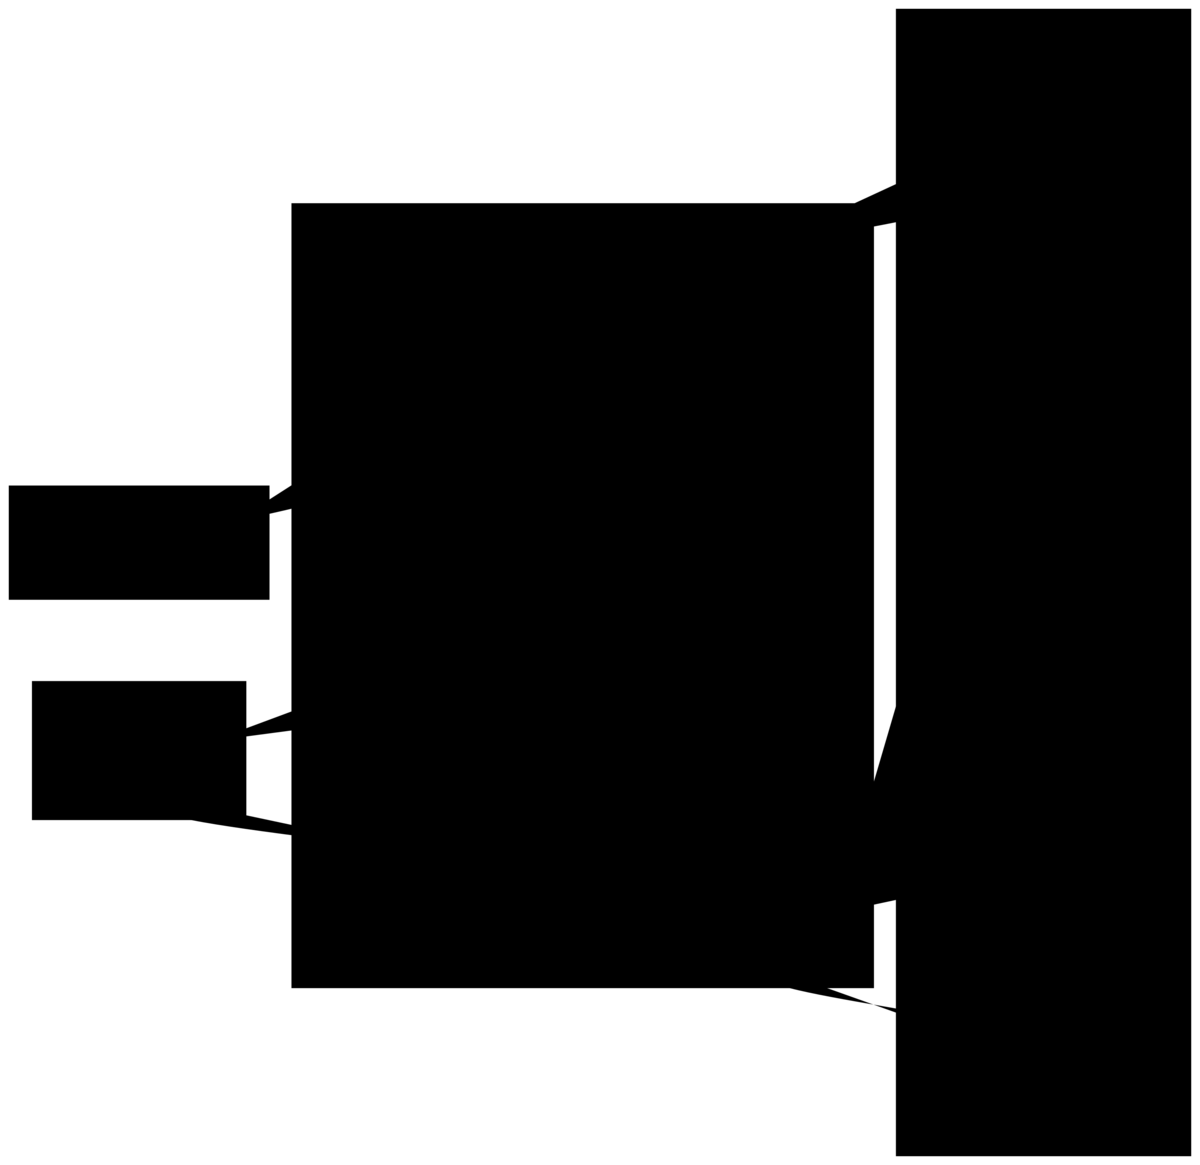
\includegraphics[width=0.95\textwidth]{img/architecture.png}
    \caption{系统总体架构图}
    \label{fig:architecture}
\end{figure}


\newpage

\section{系统分析}


\begin{figure}[H]
    \centering
    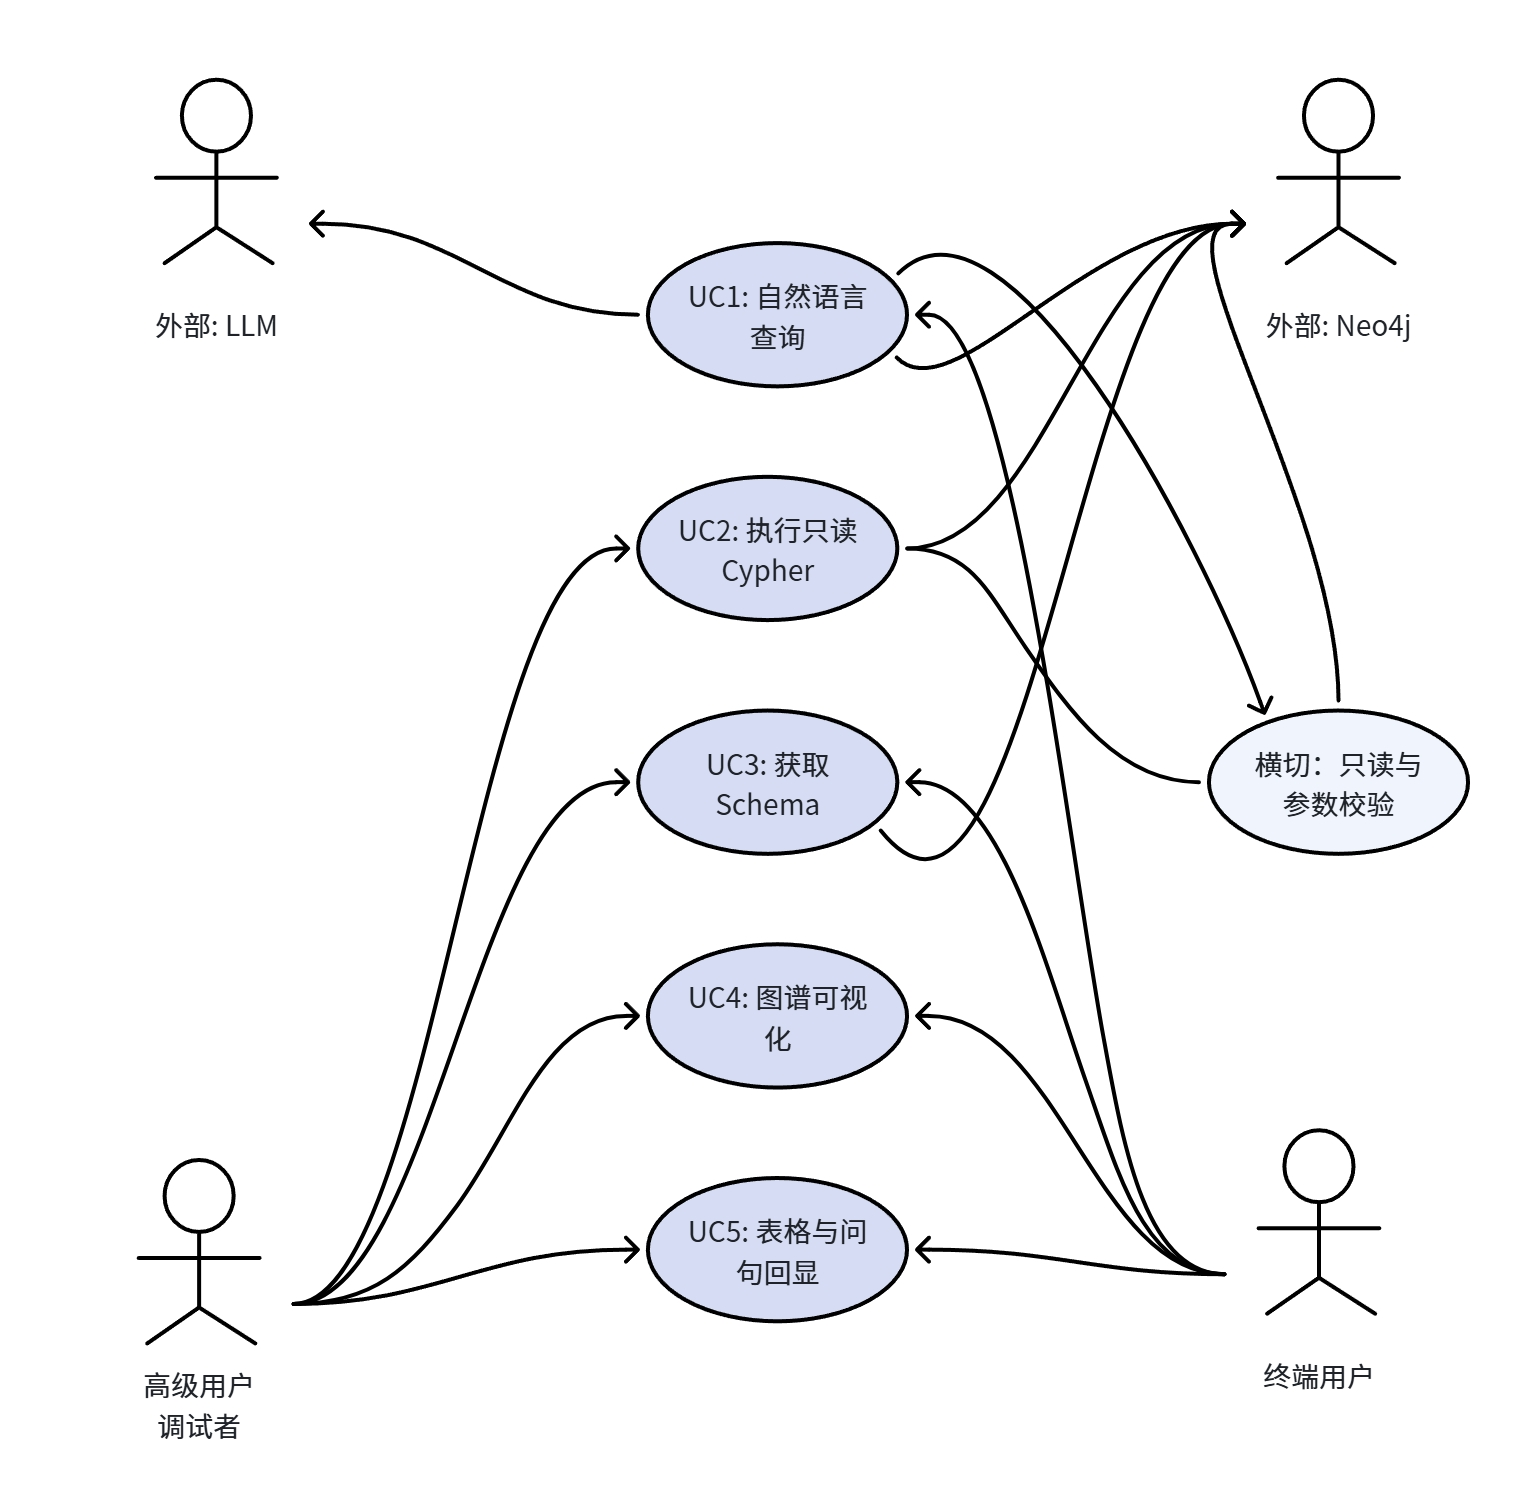
\includegraphics[width=0.95\textwidth]{img/use-case-diagram.jpg}
    \caption{系统用例图}
    \label{fig:use-case-placeholder}
\end{figure}



\begin{table}[H]
    \centering
    \caption{核心用户故事}
    \label{tab:user-stories}
    \small
    \begin{tabular}{p{1.1cm}p{4.6cm}p{5.8cm}}
        \toprule
        \textbf{编号} & \textbf{用户故事} & \textbf{验收要点} \\
        \midrule
        US-1 & 作为终端用户，我希望用中文自然语言描述查询意图，以便无需编写 Cypher 即可探索知识图谱。 & \texttt{POST /nlq} 返回 200 时含可渲染的 \texttt{graph}/\texttt{table} 与回显的生成语句；非法或危险语句被拦截。 \\
        US-2 & 作为高级用户，我希望在“Cypher”模式下直接提交只读查询，以便复现、对比自然语言生成的语句。 & \texttt{POST /run-cql} 与 NL 链路共用同一套校验与执行语义；参数化占位符与请求体一致时执行成功。 \\
        US-3 & 作为终端用户，我希望查询结果以力导向关系图展示，以便直观看到实体之间的路径与关联。 & 响应体 \texttt{graph.nodes/links} 可被前端 ECharts 正确解析；支持拖拽、缩放等基本交互。 \\
        US-4 & 作为终端用户，我希望同时看到表格化属性，以便阅读长文本或数值字段。 & 同一响应中 \texttt{table} 与图谱分区展示；列键与记录一致。 \\
        US-5 & 作为高级用户或终端用户，我希望查看当前库的Schema 摘要，以便理解可问的标签与关系类型。 & \texttt{GET /schema} 返回可供前端或人工阅读的摘要；NL 链路在生成前拉取 Schema。 \\
        US-6 & 作为系统运维方，我希望对外暴露的执行通道默认拒绝写操作与危险调用，以便在误配置账号或模型异常时仍守住安全底线。 & 黑名单关键字与参数校验对 \texttt{/nlq}、\texttt{/run-cql} 均生效；写类语句返回明确错误。 \\
        \bottomrule
    \end{tabular}
\end{table}

\newpage

\section{系统设计}

\begin{figure}[H]
    \centering
    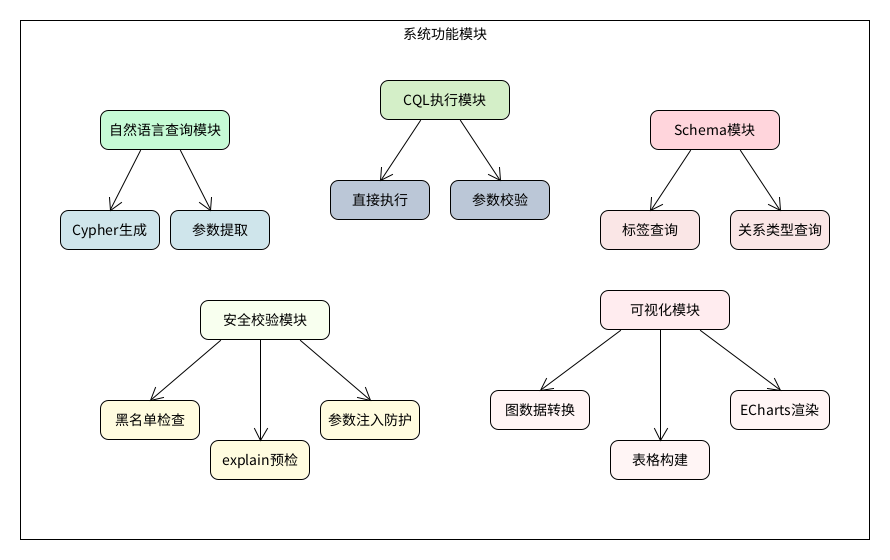
\includegraphics[width=0.95\textwidth]{img/modules.png}
    \caption{系统功能模块图}
    \label{fig:modules}
\end{figure}


\begin{figure}[H]
    \centering
    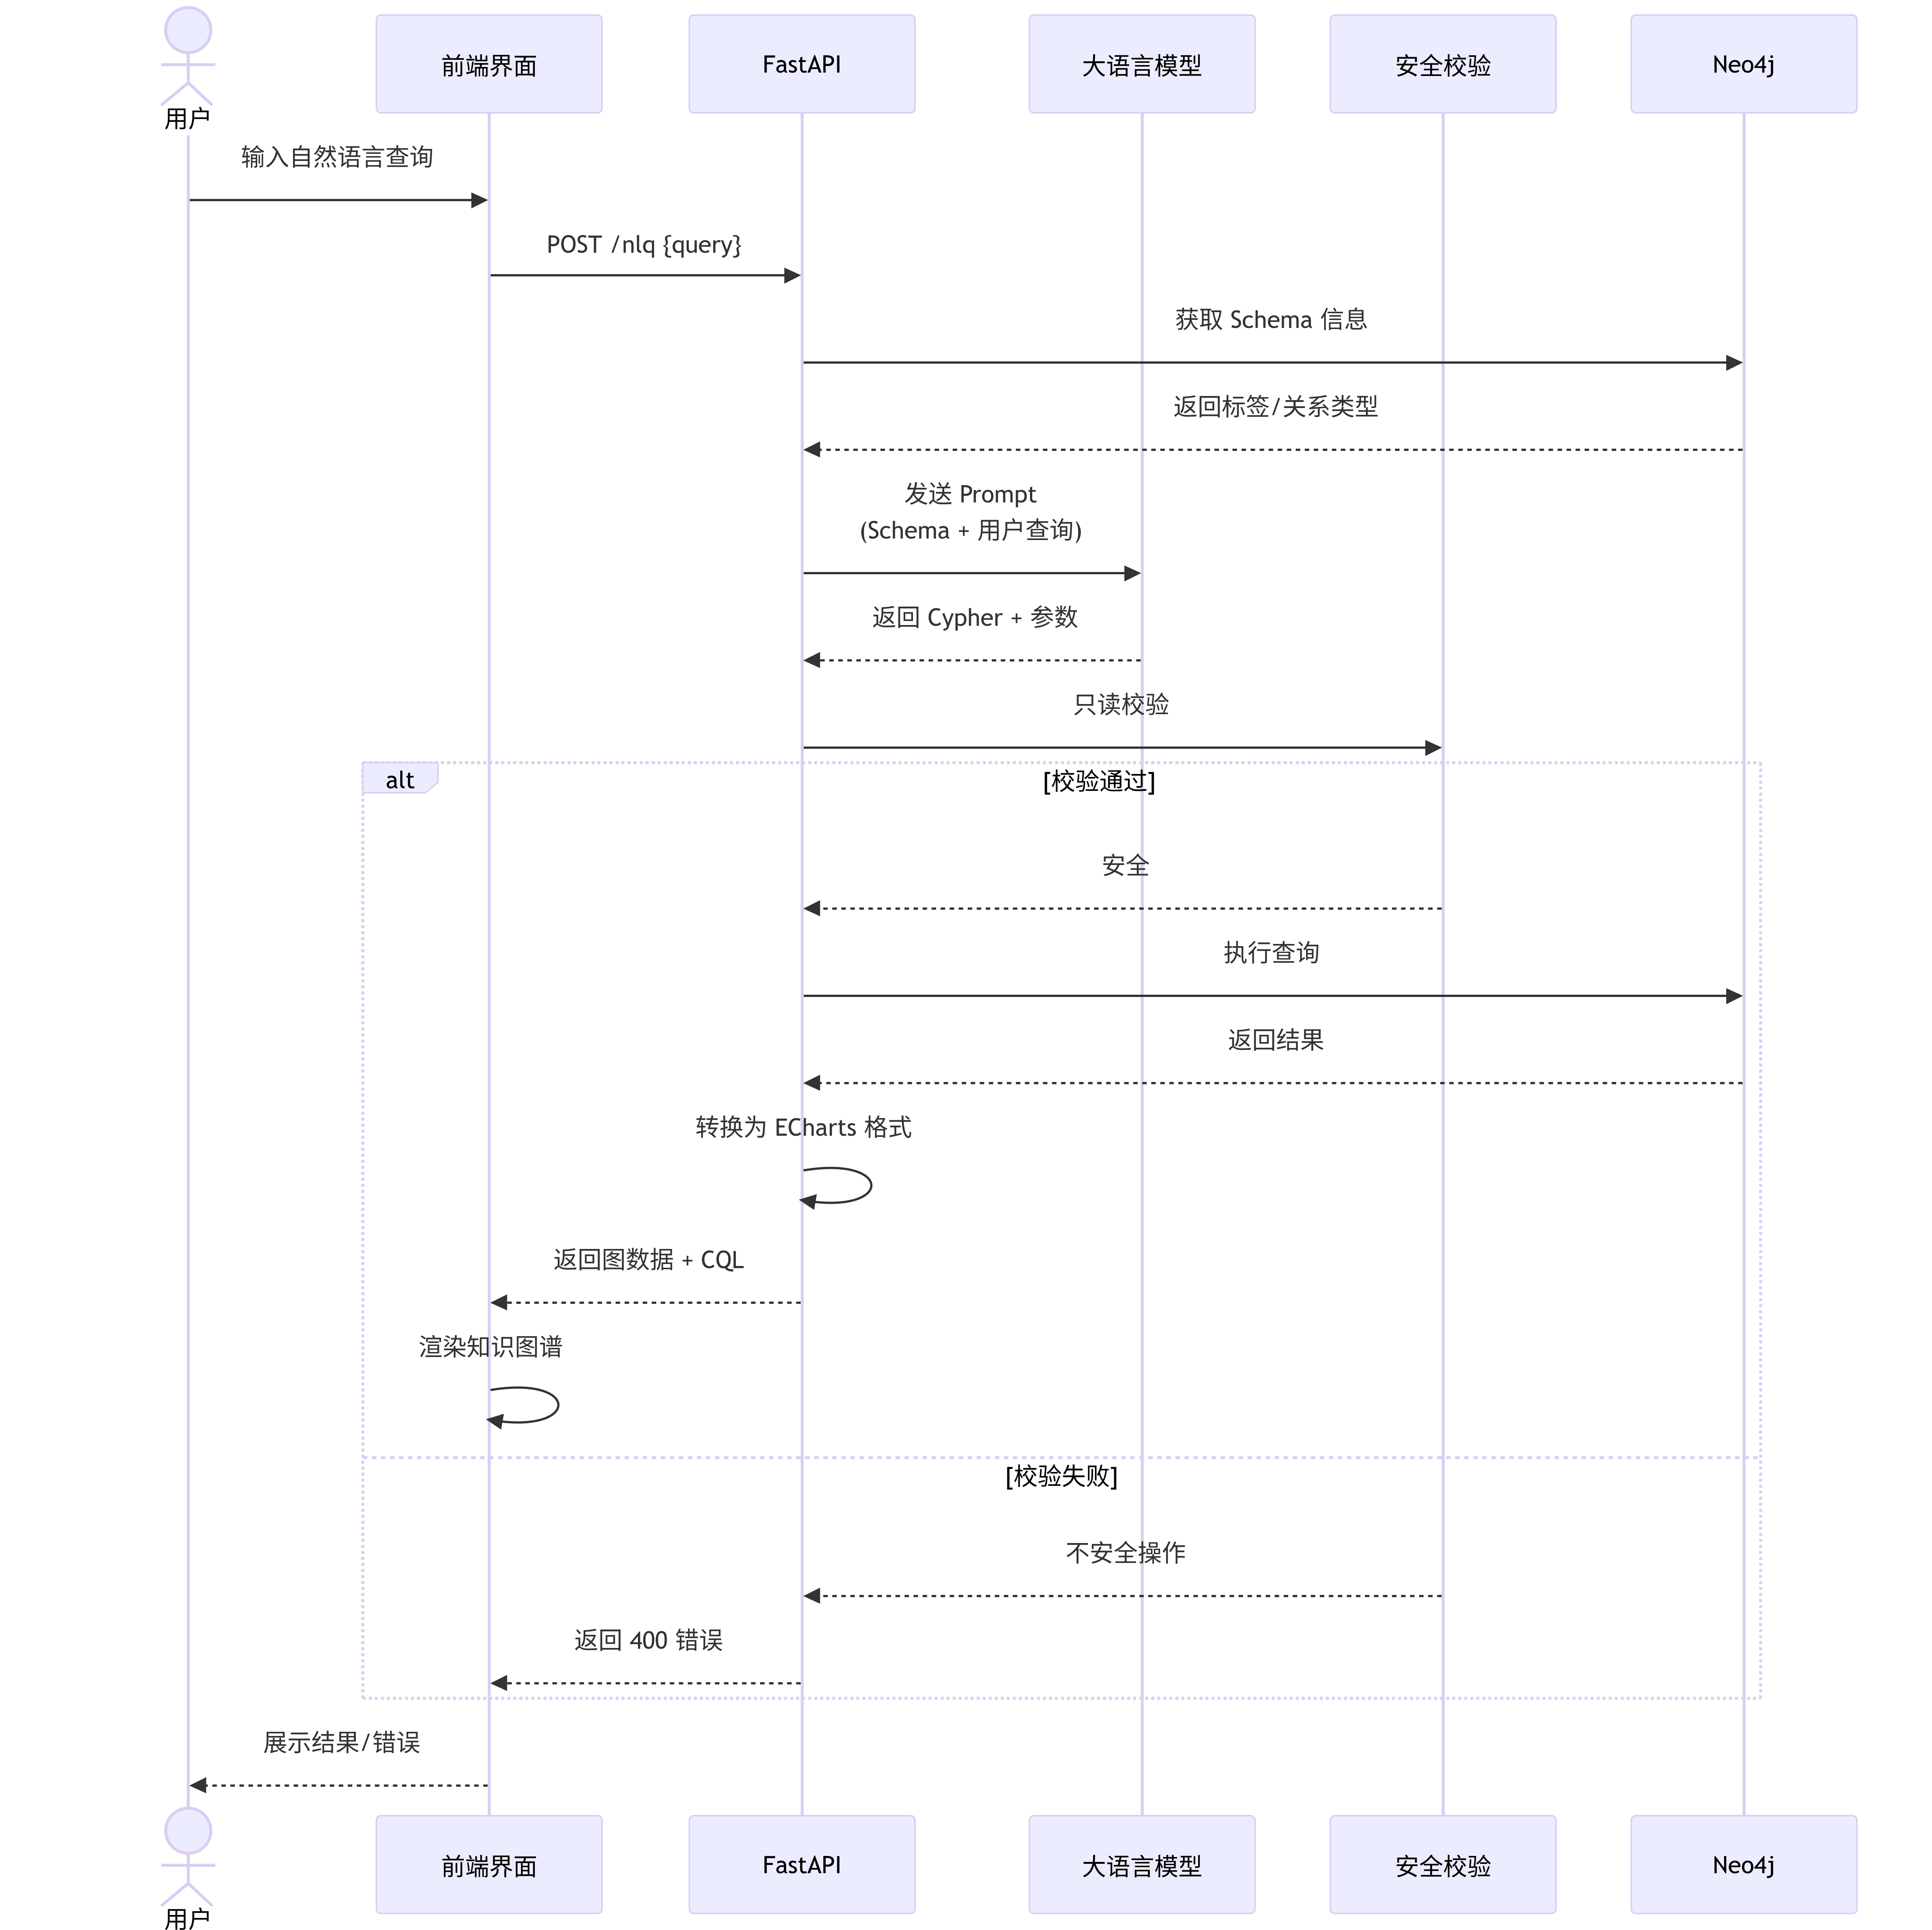
\includegraphics[width=0.95\textwidth]{img/nlq-flow.png}
    \caption{自然语言查询时序图}
    \label{fig:nlq-flow}
\end{figure}


\begin{figure}[H]
    \centering
    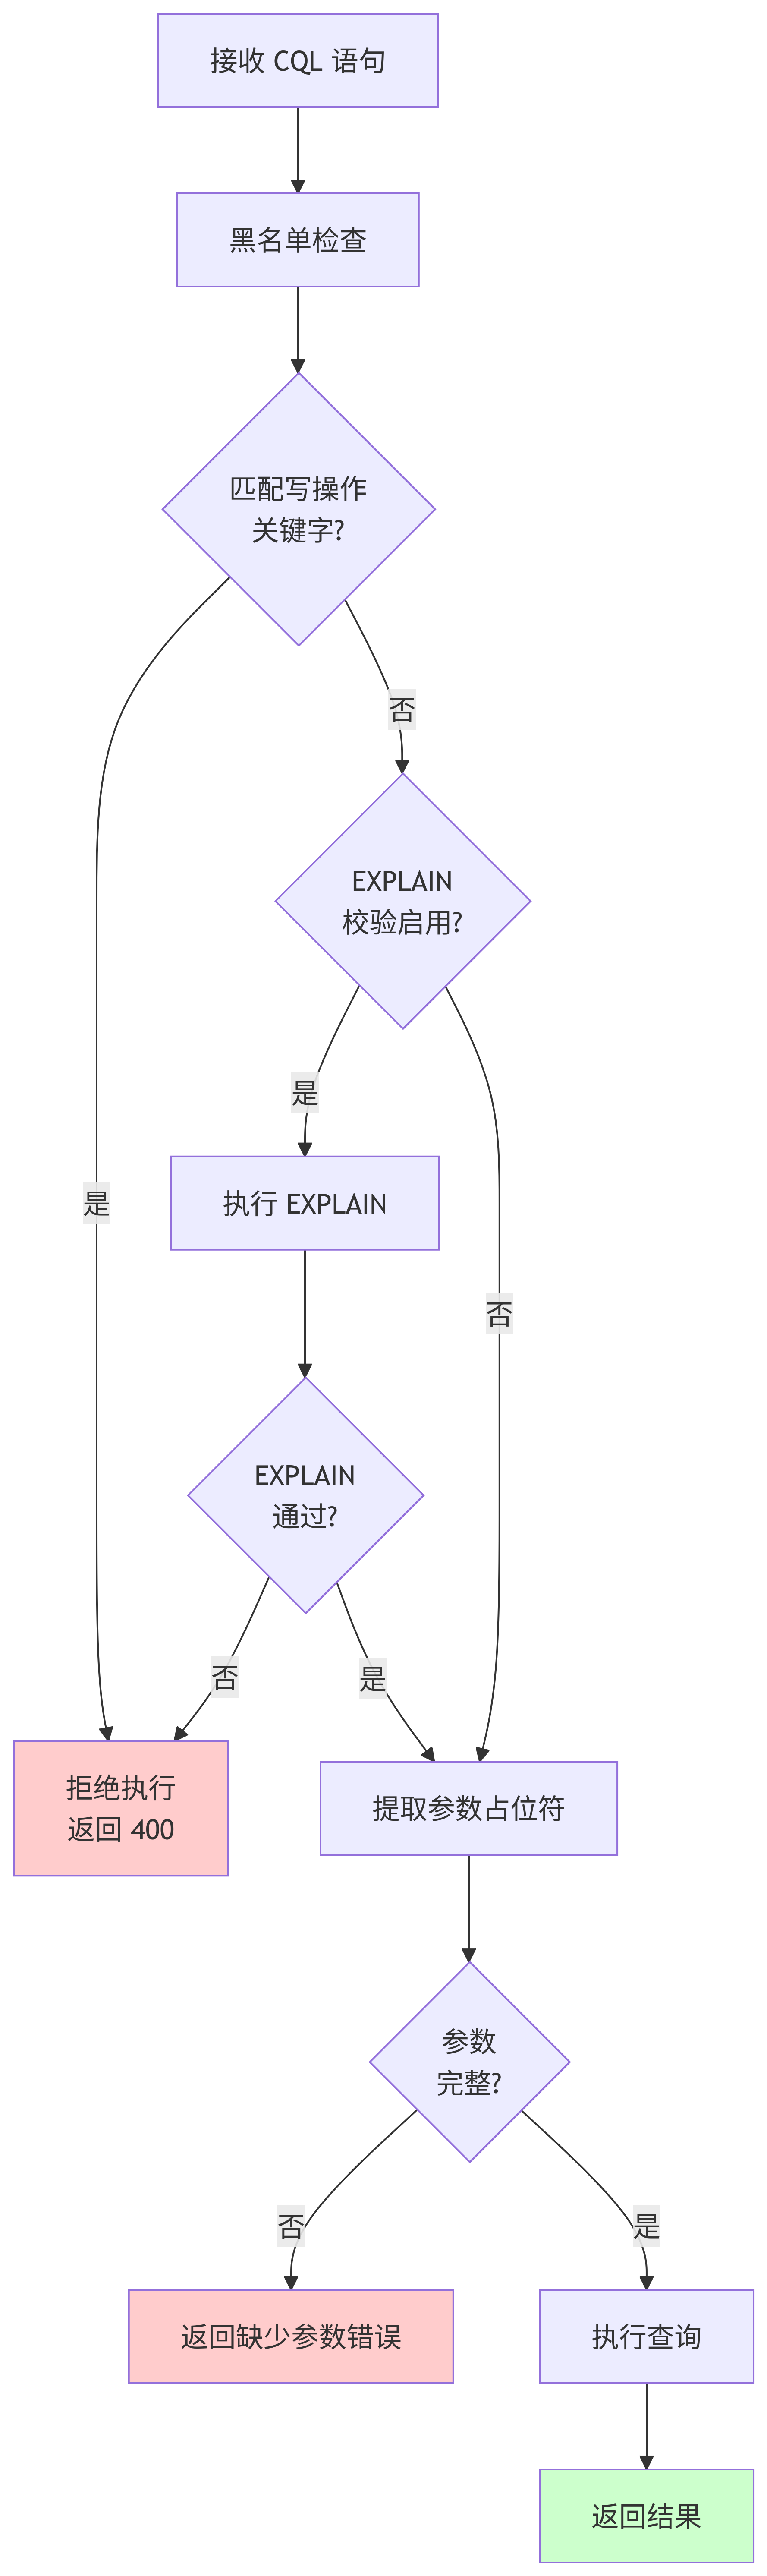
\includegraphics[width=0.8\textwidth]{img/security-flow.png}
    \caption{安全校验流程图}
    \label{fig:security-flow}
\end{figure}


\begin{figure}[H]
    \centering
    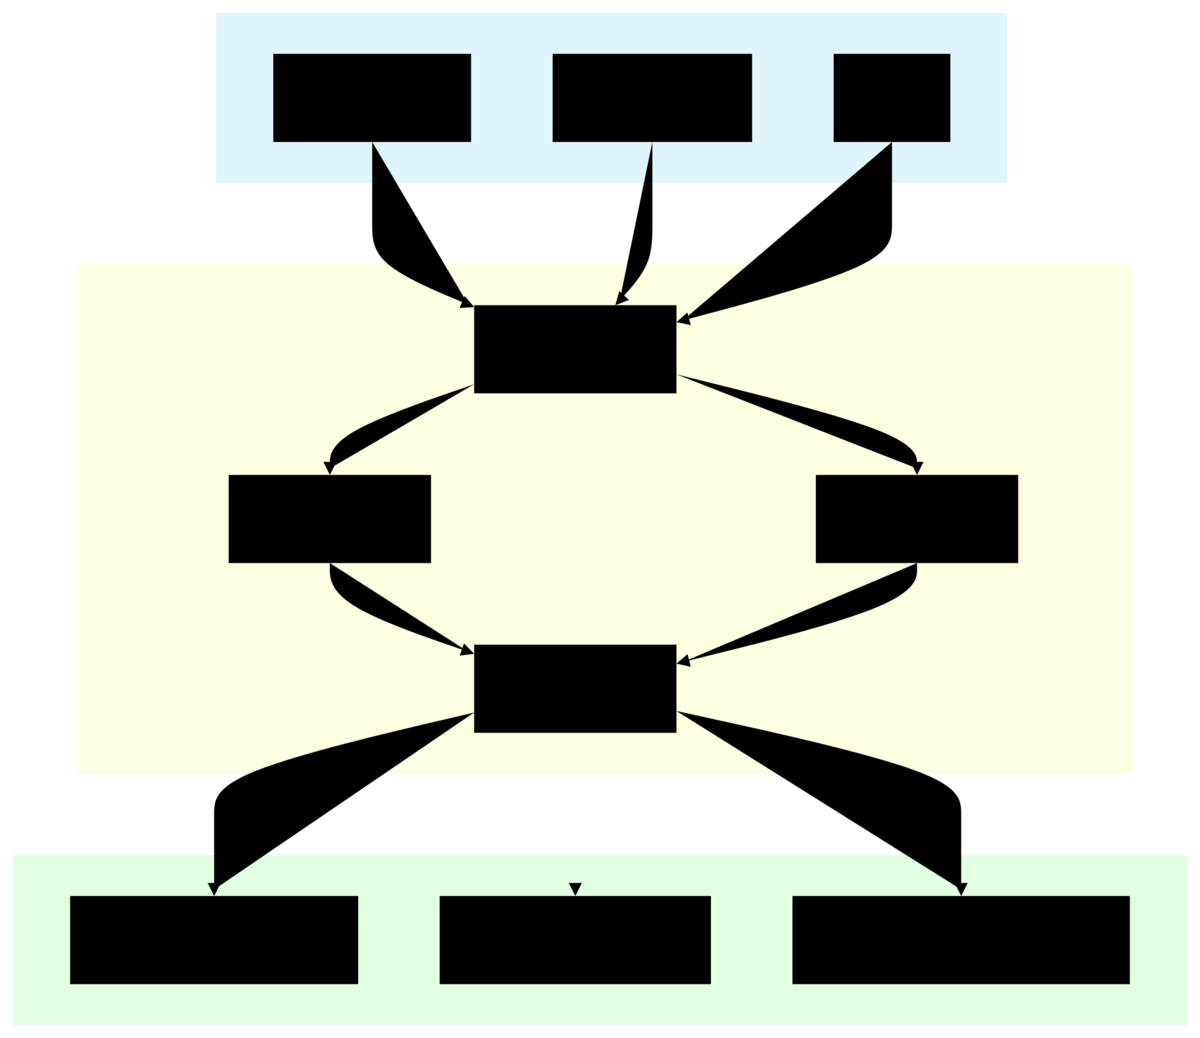
\includegraphics[width=0.9\textwidth]{img/data-convert.png}
    \caption{图数据转换流程}
    \label{fig:data-convert}
\end{figure}

\subsection{数据库设计}
\label{subsec:db-design}

本系统使用 Neo4j 图数据库存储《迷你世界》知识图谱，采用多标签属性图模型。为避免术语歧义，这里先说明本文中的两个领域词：方块指游戏世界中可采集或可放置的地形/材料单元，生物指可交互实体（如动物、怪物或 NPC）。数据库设计充分利用 Neo4j 的多标签特性，将方块和生物作为“道具”这一上位概念的子类，通过复合标签表达继承关系。

数据库设计直接影响自然语言查询和可视化效果。Schema 中的标签与关系类型会进入自然语言模块的提示词，节点上的 \texttt{Name}、\texttt{MineTool} 等属性会影响模型生成 \texttt{WHERE} 条件，也会影响转换模块如何归类节点和生成表格列。因此，数据建模不是孤立的存储设计，而是与查询体验和展示效果联动的整体设计。

\subsubsection{架构演进}

早期曾考虑兼容阿里云 GDB（Graph Database）等不支持同一节点多标签的图引擎。在该约束下，无法直接使用 \texttt{:item:block}、\texttt{:item:monster} 这类复合标签表达“方块/生物是一种道具”的继承语义，只能将方块、生物与通用道具拆成不同节点，再通过业务 ID 用桥接关系（即额外增加的中间节点或关系，用于在语义上等效继承，而非图数据库原生的多标签机制；历史上曾建模为 PLACE、SUMMON 等）与道具节点相连。

该单标签桥接方案会拉长查询路径。自然语言转 Cypher 时，模型需要记住“先找道具，再经 PLACE 或 SUMMON 跳到方块/生物”的固定模式，生成错误的概率随之上升。同时，这种建模与用户对“方块和生物也是道具类别”的直观理解不一致，维护成本较高。

当前实现已取消 GDB 兼容路径，数据仅面向 Neo4j 导入与查询。方块与生物直接采用多标签节点建模，不再使用 PLACE、SUMMON 等桥接关系。提示词设计与测试用例均以当前多标签模型为准。

\subsubsection{多标签架构设计}

Neo4j 允许同一节点携带多个标签（Multiple Labels）。本文以 \texttt{:item} 作为道具基类标签（通用属性含 ID、Name、Type、Disc、GetWay）；方块类节点同时使用 \texttt{:item:block}，在基类属性之外增加 MineTool、ToolLevel 等；生物类节点同时使用 \texttt{:item:monster}，增加 Life、Attack 等。具体列示见表~\ref{tab:node-types}。相较早期单标签桥接方案，多标签使 ``方块/生物属于道具'' 直接体现在标签上，查询时可写 \texttt{MATCH (n:item:block) RETURN n.Name, n.MineTool} 等语句而无需经 PLACE、SUMMON 等关系绕行，语义与领域模型一致，并减少不必要的跳转与联结开销。

\subsubsection{E-R图}

实体—关系图（Entity--Relationship Diagram，简称 E-R 图）在传统教材中多用于关系型表结构设计。本文图~\ref{fig:er-diagram}借用该图示习惯概括领域实体与联系；底层存储为 Neo4j 属性图，而非将每条记录展开为关系表中的行。需要说明的是，图中画法与传统关系型数据库（表、主键、外键）的书写习惯不同：本文采用“节点标签 + 关系类型”的表示法，图中使用复合标签表示继承关系，如 \texttt{:item:block} 表示“同时具有 \texttt{:item} 与 \texttt{:block} 标签的节点”，即方块继承道具的通用属性并增加专属属性。

\begin{figure}[H]
    \centering
    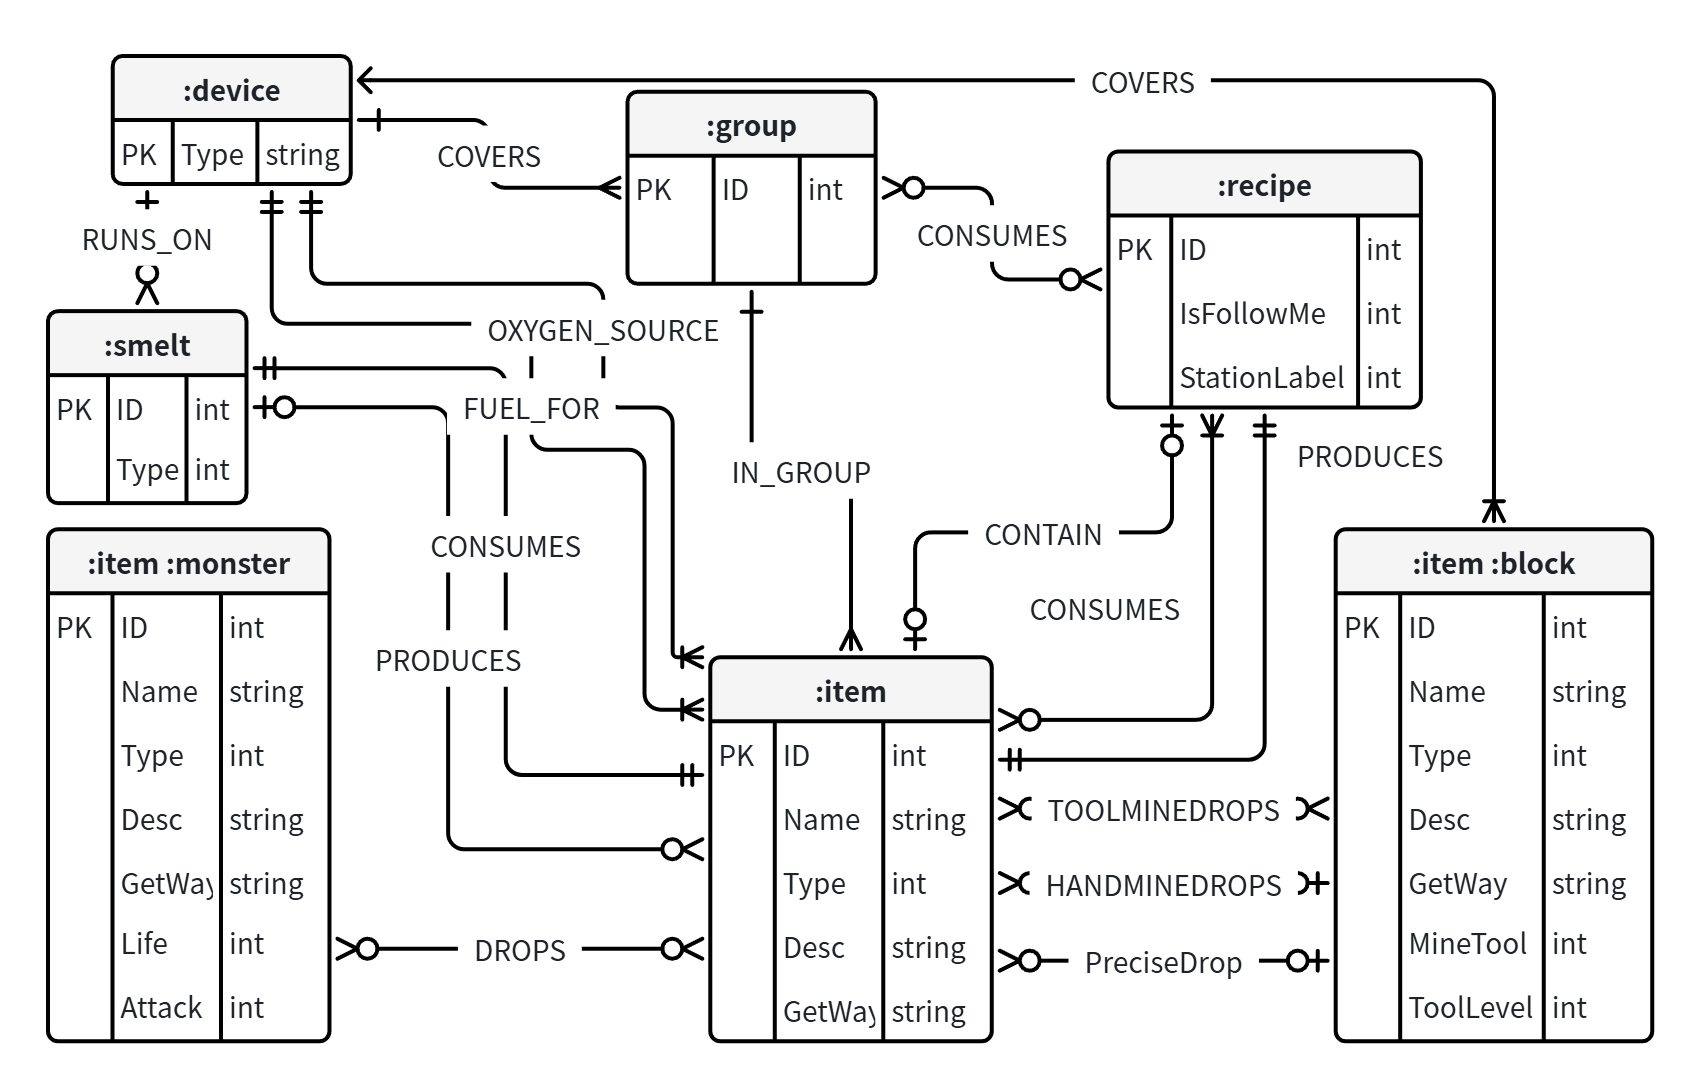
\includegraphics[width=0.95\textwidth]{img/er-diagram.jpg}
    \caption{知识图谱E-R图}
    \label{fig:er-diagram}
\end{figure}

\subsubsection{节点类型}

为帮助读者从关系型数据库思维过渡到图数据库思维，表~\ref{tab:node-types}中的“标签”列并非关系表名，而是 Neo4j 节点类型标识。以 \texttt{:item} 为例，前导冒号是 Cypher 中“标签”的语法；\texttt{:item:block} 表示同一节点可带多个标签，而不是两张表做联结后的结果。

\begin{table}[H]
    \centering
    \caption{节点类型及属性}
    \label{tab:node-types}
    \begin{tabular}{llp{8cm}}
        \toprule
        \textbf{标签} & \textbf{说明} & \textbf{属性} \\
        \midrule
        :item & 游戏道具（基类） & ID, Name, Type, Disc, GetWay \\
        :item:block & 方块（继承:item） & +MineTool, ToolLevel \\
        :item:monster & 生物（继承:item） & +Life, Attack \\
        :group & 物品分组 & ID \\
        :recipe & 合成配方 & ID, IsFollowMe, StationLabel \\
        :smelt & 熔炼流程 & ID, Type \\
        :device & 设备抽象 & type \\
        \bottomrule
    \end{tabular}
\end{table}

\subsubsection{关系类型}

\begin{table}[H]
    \centering
    \caption{关系类型及说明}
    \label{tab:rel-types}
    \begin{tabular}{lll}
        \toprule
        \textbf{关系类型} & \textbf{起点} & \textbf{终点} \\
        \midrule
        IN\_GROUP & (:item) & (:group) \\
        CONSUMES & (:recipe) & (:item / :item:block / :group) \\
        PRODUCES & (:recipe) & (:item / :item:block) \\
        CONTAIN & (:recipe) & (:item) \\
        HANDMINEDROPS & (:item:block) & (:item) \\
        TOOLMINEDROPS & (:item:block) & (:item) \\
        PreciseDrop & (:item:block) & (:item) \\
        DROPS & (:item:monster) & (:item) \\
        COVERS & (:device) & (:group|:item:block) \\
        RUNS\_ON & (:smelt) & (:device) \\
        FUEL\_FOR & (:item) & (:device) \\
        OXYGEN\_SOURCE & (:item) & (:device) \\
        \bottomrule
    \end{tabular}
\end{table}

\subsubsection{数据规模}

本系统使用的知识图谱数据规模如表~\ref{tab:data-scale}所示。表中各类节点按互斥口径统计：占比列为占节点总计的百分比，设备类因数量极少写作``$<$0.1\%''。关系条数按 Neo4j 中有向关系实例计数；读者可用 \texttt{MATCH ()-[r]->() RETURN count(r)} 在库内复核，与导入脚本一致。

\begin{table}[H]
    \centering
    \caption{知识图谱数据规模}
    \label{tab:data-scale}
    \begin{tabular}{lcc}
        \toprule
        \textbf{类型} & \textbf{数量} & \textbf{占比} \\
        \midrule
        纯物品(:item，不含:block/:monster) & 3,514 & 45.2\% \\
        方块(:item:block) & 1,936 & 24.9\% \\
        生物(:item:monster) & 262 & 3.4\% \\
        配方(:recipe) & 1,961 & 25.3\% \\
        分组(:group) & 65 & 0.8\% \\
        熔炼(:smelt) & 25 & 0.3\% \\
        设备(:device) & 3 & $<$0.1\% \\
        \midrule
        \textbf{节点总计} & \textbf{7,766} & 100\% \\
        \midrule
        关系总计 & 12,240 & - \\
        \bottomrule
    \end{tabular}
\end{table}

\subsection{本章小结}

设计原则概括为职责分离、横切安全与可观测性；总体架构以分层方式划分浏览器页面、FastAPI 业务层、Neo4j 访问层与大语言模型外部服务。核心功能模块按请求进入、语句校验、数据库执行与结果展示的顺序衔接；数据库设计说明多标签模型、实体—关系图示、节点与关系类型及数据规模，并阐明 Schema 对自然语言查询与可视化的约束。上述内容为第~\ref{sec:detailed-implementation}~章详细实现与测试验收提供直接依据。

\newpage

\section{详细设计与实现}
\label{sec:detailed-implementation}

本章说明系统结构与数据模型如何落实为可运行代码：浏览器或脚本通过 HTTP 访问统一的服务地址（下文称端点），例如用 GET 拉取页面与健康状态、用 POST 提交自然语言或 Cypher；后端据此完成自然语言编排或直接执行只读查询，语句在进入 Neo4j 前经过安全约束，出库记录再转换为前端可展示的图与表。

正文按四个核心模块编排，共用接口见表~\ref{tab:api}。自然语言链路与直接 Cypher 链路在进入数据库前共用同一套安全校验与 Neo4j 执行封装，与图~\ref{fig:modules}中的模块划分一致。下文以``查找石剑''的 \texttt{POST /nlq} 为例，说明路由、校验与转换步骤。

\begin{table}[H]
    \centering
    \caption{系统API接口列表}
    \label{tab:api}
    \begin{tabular}{llll}
        \toprule
        \textbf{方法} & \textbf{端点} & \textbf{功能} & \textbf{认证} \\
        \midrule
        GET & / & 返回Web前端页面（\texttt{index.html}） & 否 \\
        GET & /health & 健康检查 & 否 \\
        GET & /schema & 获取Schema信息 & 否 \\
        POST & /run-cql & 执行Cypher查询 & 否 \\
        POST & /nlq & 自然语言查询 & 否 \\
        \bottomrule
    \end{tabular}
\end{table}

表~\ref{tab:api}中``方法''列：GET 多用于读取页面或元数据，POST 多用于携带 JSON 正文提交待执行内容。``认证''列在本仓库演示版本中均为``否''，表示应用内未集成登录与令牌校验；课程或内网演示可直接使用，若面向公网部署，宜在网关、反向代理或独立认证服务侧另行接入身份校验，而非仅依赖本表所列端点。

\subsection{自然语言查询模块的设计与实现}
\label{subsec:nlq-impl}

自然语言查询模块负责将中文问句映射为参数化、只读、便于路径可视化的 Cypher。为使模型生成结果与当前图库一致，后端在调用大语言模型（Large Language Model, LLM）前先拉取 Schema 摘要，并将其与用户问句一并写入提示词（即将约束说明与问句组合后送往模型的固定文字）。模型返回结果被约束为 JSON，主要字段为 \texttt{cql} 与 \texttt{params}，便于后续安全校验及在 Neo4j 侧按名称绑定参数取值。

对外入口为表~\ref{tab:api}中的 \texttt{POST /nlq}。实现上，FastAPI 根据 URL 路径将请求分发至对应处理函数（路由），编排``取 Schema、调用 \texttt{llm\_client.generate\_cypher}、进入安全模块、访问 Neo4j、调用转换器''的流水线。以下给出请求与响应的数据形状，与时序图~\ref{fig:nlq-flow}一致。

请求体格式：
\begin{lstlisting}[language=json, caption={自然语言查询请求体}]
{
    "query": "查找石剑",
    "options": {
        "limit": 100,
        "debug_raw": false
    }
}
\end{lstlisting}

响应体格式（字段名 \texttt{cql} 为历史命名，内容为Cypher字符串）：
\begin{lstlisting}[language=json, caption={自然语言查询响应体}]
{
    "cql": "MATCH (n:item) WHERE n.Name CONTAINS $name RETURN n",
    "params": {"name": "石剑"},
    "graph": {
        "nodes": [...],
        "links": [...],
        "categories": [...]
    },
    "table": {...}
}
\end{lstlisting}

提示词与生成策略可概括为四点：限定只读查询，注入当前库 Schema，说明多标签与路径式 \texttt{RETURN path} 的使用方式，并要求输出 JSON。仅返回孤立节点时，前端难以恢复边信息，因此提示词倾向于引导模型返回路径。完整标签、关系类型、多组少样本示例（文献与工程中常称 few-shot，即在提示词中给出少量输入输出范例）与调参说明见附录\ref{app:prompt-supplement}。正文仅保留一个代表性示例：
\begin{lstlisting}[language=cypher, caption={合成问句与路径式返回（与附录中其余少样本示例同型）}]
-- 木料能合成什么
MATCH path = (material:item)-[:CONSUMES]-(r:recipe)-[:PRODUCES]-(product:item)
WHERE material.Name CONTAINS '木料'
RETURN path LIMIT 20
\end{lstlisting}

调用与解析的实现摘录如下。自然语言模块将系统提示词与用户问句拼装为 OpenAI 兼容的对话补全接口请求（路径通常为 \texttt{/chat/completions}），并要求响应体为 JSON，以便提取 \texttt{cql} 与 \texttt{params}。

\begin{lstlisting}[language=Python, caption={LLM 生成 Cypher（llm\_client.py 摘录）}]
async def generate_cypher(self, nlq, schema_hint, limit):
    payload = {
        "model": self.model,
        "messages": [
            {"role": "system", "content": load_system_prompt()},
            {"role": "user", "content": f"只读 Cypher，LIMIT 默认 {limit}：\n{nlq}"},
        ],
        "temperature": 0.1,
        "response_format": {"type": "json_object"},
    }
    resp = await client.post(f"{self.api_base}/chat/completions", json=payload, headers=headers)
    obj = json.loads(resp.json()["choices"][0]["message"]["content"])
    return obj.get("cql", "").strip(), obj.get("params", {})
\end{lstlisting}

\subsection{图数据访问与 Cypher 执行模块的设计与实现}

图数据访问与 Cypher 执行模块将最终进入数据库的查询收敛到统一的 Neo4j 客户端封装。会话使用只读访问模式（Neo4j 驱动层面对会话施加读权限标记），查询携带数据库名与超时配置，返回记录字典与列键序，供转换模块继续处理。\texttt{GET /schema} 为自然语言链路和人工浏览提供标签、关系摘要；\texttt{POST /run-cql} 为高级用户提供与自然语言入口相同的执行语义；\texttt{GET /health} 供部署脚本或编排系统周期性访问，以判断进程是否存活（健康检查）。路由层在通过 \texttt{cql\_validator} 校验后才调用 \texttt{run\_read}。下列代码摘录展示只读会话与超时换算。

\begin{lstlisting}[language=Python, caption={Neo4j 只读查询（neo4j\_client.py 摘录）}]
def run_read(self, cql: str, params: Dict[str, Any] | None = None):
    params = params or {}
    with self._driver.session(
        database=settings.NEO4J_DATABASE,
        default_access_mode="READ",
    ) as session:
        timeout_seconds = settings.QUERY_TIMEOUT_MS / 1000.0
        result = session.run(cql, parameters=params, timeout=timeout_seconds)
        records = [r.data() for r in result]
        return records, list(result.keys())
\end{lstlisting}

仓库内 \texttt{pytest} 对 API 与校验器做契约级验证（即用断言检验路径、HTTP 状态码与响应 JSON 字段是否与约定一致）。终端测试用例全部通过时的输出示例见图~\ref{fig:screenshot-pytest}；测试范围与断言口径见第~\ref{sec:system-test}~章。

\begin{figure}[H]
    \centering
    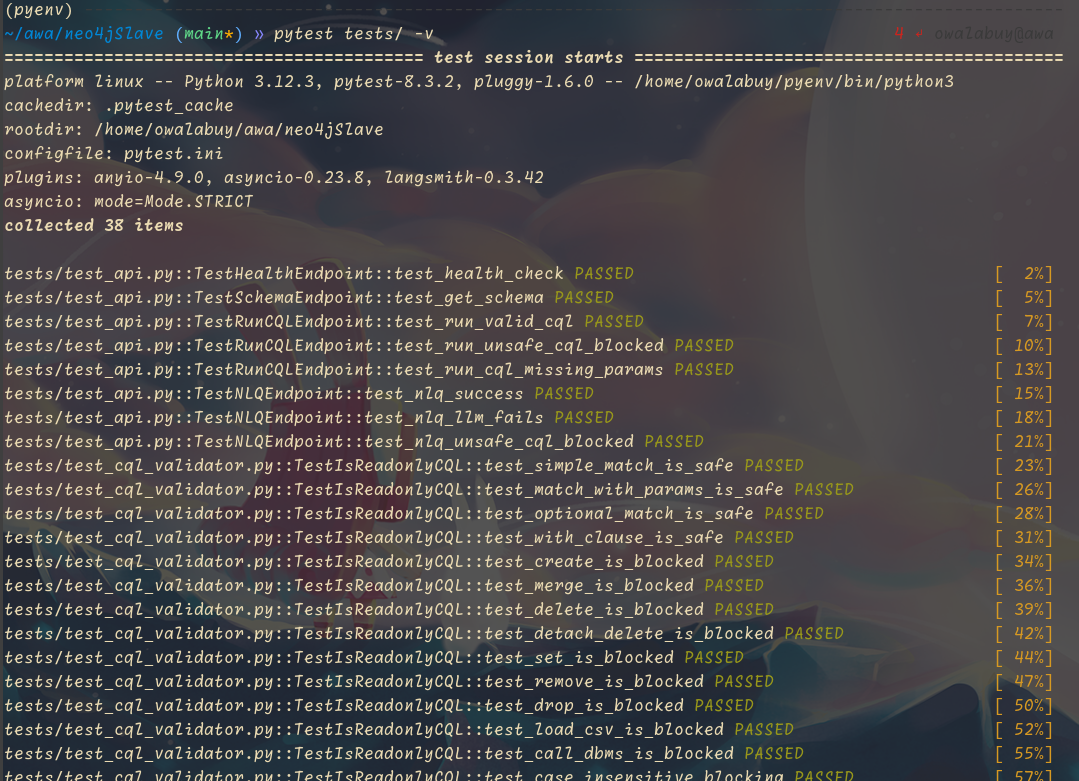
\includegraphics[width=0.95\textwidth]{img/pytest-run.png}
    \caption{自动化测试运行截图}
    \label{fig:screenshot-pytest}
\end{figure}

\subsection{结果转换与可视化模块的设计与实现}

Neo4j 驱动返回的记录可能同时包含节点、关系和路径对象，而 ECharts 的关系图组件需要统一的 \texttt{nodes}/\texttt{links} 结构（节点列表及连接两端的有向边列表）。因此，后端在 JSON 响应中并行返回 \texttt{graph} 与 \texttt{table}，使前端既能展示拓扑，也能展示属性。转换过程主要包括遍历记录、识别节点和关系、生成唯一节点 ID、提取关系端点、去重节点以及处理仅有节点而无边的退化情形。核心逻辑位于 \texttt{echarts\_converter.py}；下列摘录展示关系边入库时如何保证端点节点先行入表。

\begin{lstlisting}[language=Python, caption={图数据转换（echarts\_converter.py 摘录）}]
def add_rel(rel: graph.Relationship) -> None:
    src, tgt = _node_id(rel.start_node), _node_id(rel.end_node)
    add_node(rel.start_node)
    add_node(rel.end_node)
    links.append({
        "source": src, "target": tgt,
        "category": rel.type, "label": rel.type,
        "value": dict(rel),
    })
\end{lstlisting}

前端采用单页面设计，包括查询输入区、图谱展示区、表格展示区和生成语句回显区。界面总览见图~\ref{fig:webui}；自然语言查询端到端效果见图~\ref{fig:screenshot-nlq}。

\begin{figure}[H]
    \centering
    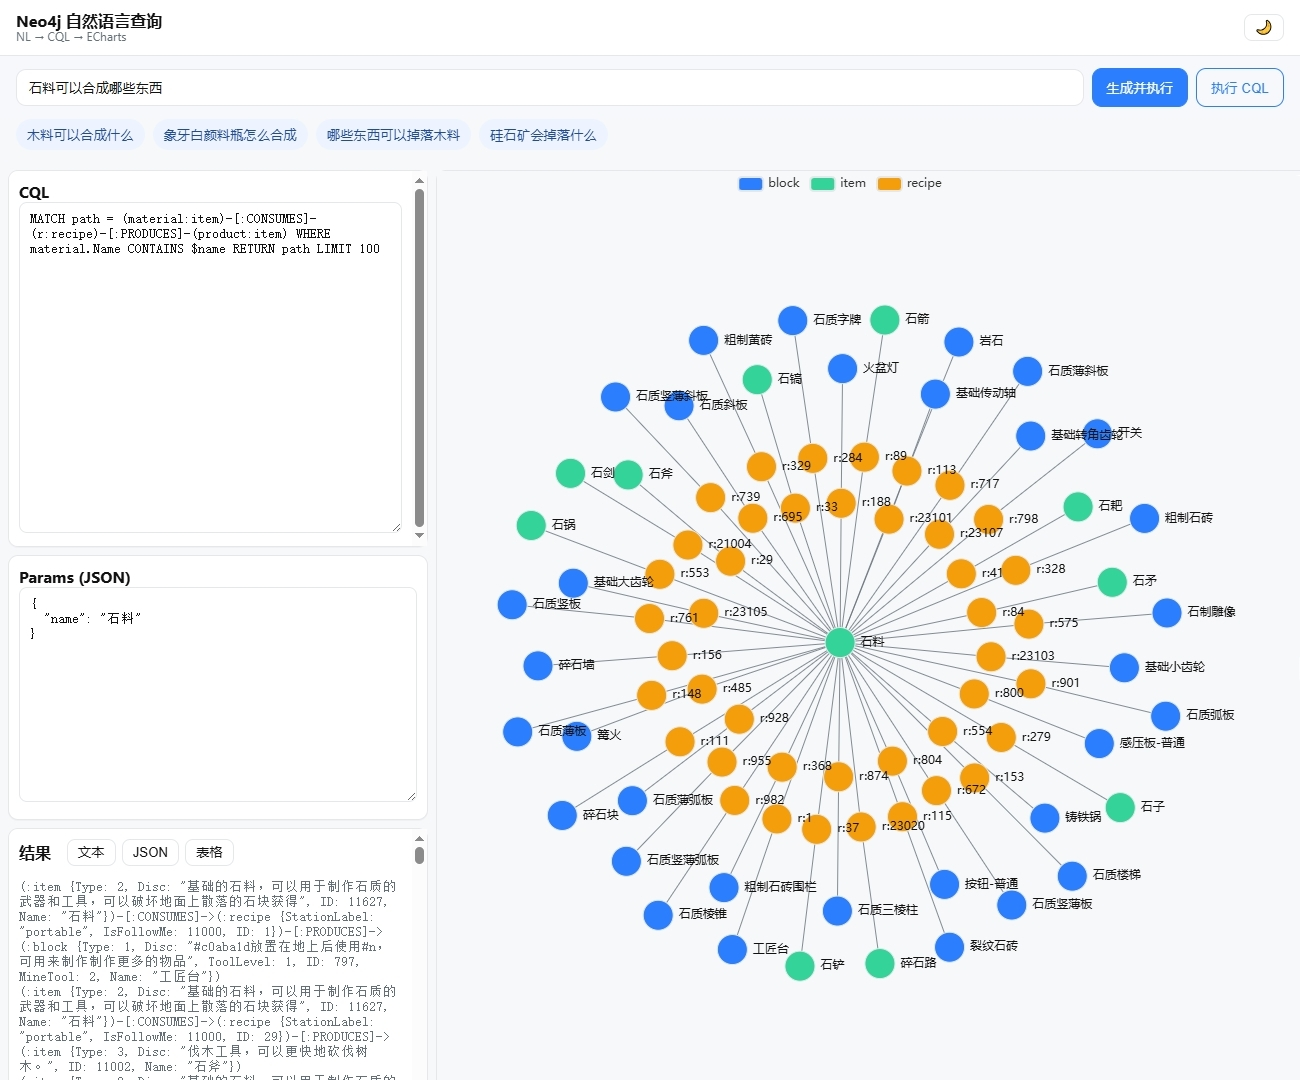
\includegraphics[width=0.95\textwidth]{img/webui.jpg}
    \caption{系统前端界面运行截图}
    \label{fig:webui}
\end{figure}

\begin{figure}[H]
    \centering
    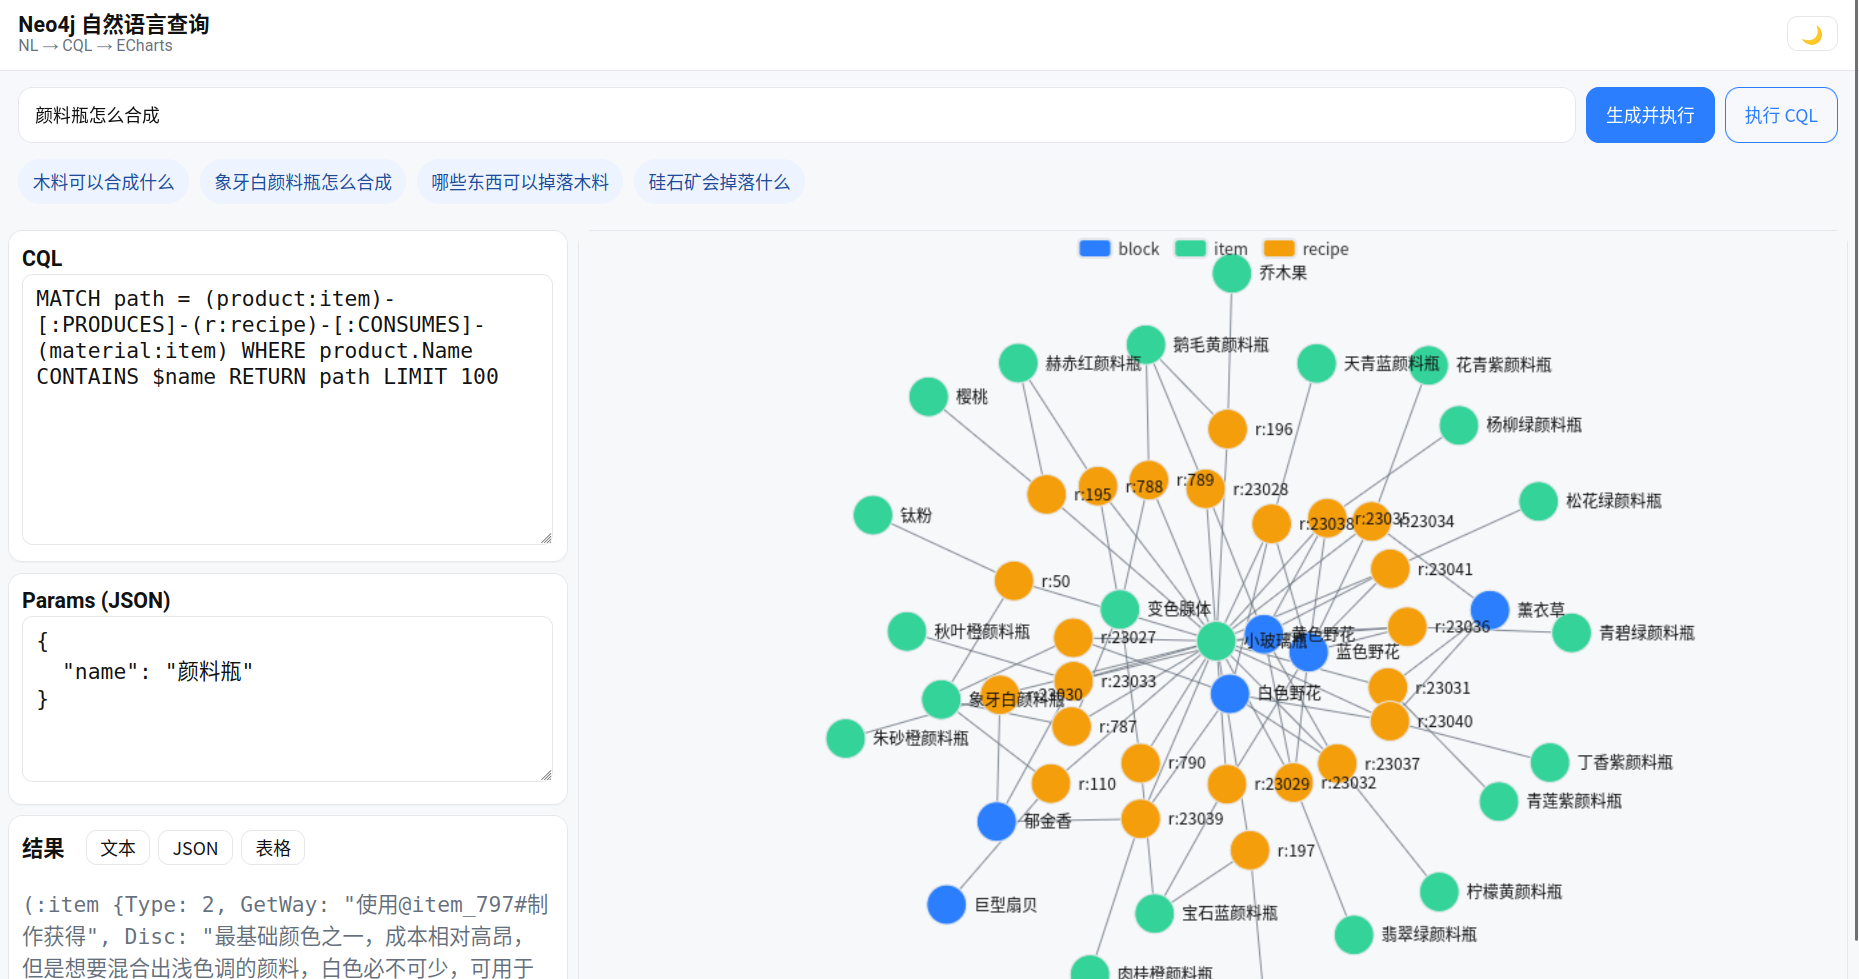
\includegraphics[width=0.95\textwidth]{img/nlq-query-result.png}
    \caption{自然语言查询结果截图}
    \label{fig:screenshot-nlq}
\end{figure}

\subsection{安全与约束模块的设计与实现}

安全模块以横切方式作用于 \texttt{/nlq} 与 \texttt{/run-cql}。在调用 Neo4j 前，系统先对语句做只读关键字黑名单匹配，再检查 \texttt{\$param} 占位符与请求体参数是否一致；可选 \texttt{EXPLAIN} 预检由配置项控制，默认关闭以降低图库负载。即便数据库账号配置为只读，应用层仍应拒绝明显写操作及 Neo4j 管理类过程调用（例如形如 \texttt{CALL dbms.*}、意在修改实例配置或执行管理命令的语句），并向调用方返回可读错误。校验逻辑集中在 \texttt{cql\_validator.py}，下列黑名单与表~\ref{tab:readonly-test} 中测试用例对应：

\begin{lstlisting}[language=Python, caption={只读校验黑名单（与 cql\_validator.py 一致）}]
WRITE_BLACKLIST = [
    r"\bCREATE\b",
    r"\bMERGE\b",
    r"\bDELETE\b",
    r"\bDETACH\s+DELETE\b",
    r"\bSET\b",
    r"\bREMOVE\b",
    r"\bDROP\s+(?:INDEX|CONSTRAINT|NODE\s+LABEL|REL\s+TYPE|PROPERTY)\b",
    r"\bLOAD\s+CSV\b",
    r"\bCALL\s+DBMS\.",
]
\end{lstlisting}

除上述关键字拦截外，系统未对 \texttt{CALL} 所调用的自定义存储过程（例如常用扩展库 APOC 提供的辅助过程）做白名单约束。部署假设为：图库以只读账号或只读副本访问；服务置于内网，或经反向代理（将对外域名与端口统一转发至内网服务地址）并配合鉴权后再暴露，从而将可执行 Cypher 的攻击面与误用面限制在可信主体内。若在不可信网络环境下对外开放接口，应另加网关层策略或扩展校验逻辑。

参数占位符与请求体一致性检验的实现要点如下：使用正则表达式提取 Cypher 中的 \texttt{\$param}，与请求体提供的参数键对照，确保必需参数齐全。\texttt{/run-cql} 与 \texttt{/nlq} 共用该逻辑；路由实现位于源码树 \texttt{backend/app/} 下，路径约定见第~\ref{subsec:repo-and-paths}~节。

\subsection{本章小结}

本章按四个核心模块给出详细设计与关键实现摘录：自然语言模块交代生成策略、请求/响应数据形状与调用代码；完整提示词与多组少样本示例见附录\ref{app:prompt-supplement}；图数据访问与执行模块统一只读会话、超时与各端点契约；结果转换与可视化模块说明记录到 \texttt{nodes}/\texttt{links} 的映射；安全与约束模块以前置校验拦截高风险语句并检查参数完整性。上述实现与第~\ref{sec:system-design}~章设计相对应；测试的组织与判定口径见第~\ref{sec:system-test}~章。

\newpage

\section{系统测试}
\label{sec:system-test}

\subsection{测试目的与方法}

本章回答两类验证问题：其一，接口契约、安全校验与结果转换是否在程序层面按约定运行；其二，在既定领域图数据上，真实中文问句经自然语言链路能否得到评判者可接受的结果。

系统测试分为自动化测试与人工走查。自动化测试使用 Python 测试框架 \texttt{pytest}，通过脚本调用后端路由并断言 HTTP 状态码与响应 JSON 是否与实现一致（下文统称接口契约）；覆盖只读黑名单、参数占位符一致性以及 Neo4j 返回记录到前端图结构的转换等逻辑。其中自然语言接口 \texttt{/nlq} 在自动化中对大语言模型的调用替换为预先设定的假返回（Mock），以避免评测依赖云端配额并保证多次运行结果可比对。人工走查则在固定模型、固定图数据与书面判定协议下进行：评判者逐条核对生成语句与查询结果是否满足协议中的通过条件，度量的是端到端可用性，而非某一函数的单元隔离测试。

两类测试回答的问题不同：自动化测试说明代码行为是否与仓库内约定一致；人工走查说明在当前模型与数据版本下自然语言入口的实际可用程度。分工、局限与可外推范围见表~\ref{tab:test-scope}。

与表~\ref{tab:nlq-category} 对应的人工走查环境与采样参数见表~\ref{tab:eval-runtime}。更换大语言模型服务端点、模型名、采样温度（temperature，控制生成结果的随机程度）或图数据导入版本后，应重新执行走查并重填统计表。自动化用例件数以仓库当前 \texttt{pytest} 收集结果为准；本文所写 38 条对应撰写时的提交版本。

\begin{table}[H]
    \centering
    \captionsetup{justification=centering, singlelinecheck=false}
    \caption[自动化与人工走查测试分工表]{自动化测试与人工走查的分工与可外推范围}
    \label{tab:test-scope}
    \small
    \setlength{\tabcolsep}{4pt}
    \begin{tabular}{>{\RaggedRight\arraybackslash}p{0.12\linewidth} >{\RaggedRight\arraybackslash}p{0.4\linewidth} >{\RaggedRight\arraybackslash}p{0.4\linewidth}}
        \toprule
        & \textbf{自动化 \texttt{pytest}} & \textbf{人工 NLQ 走查} \\
        \midrule
        主要覆盖 & \texttt{tests/test\_cql\_validator.py}：只读/黑名单/EXPLAIN 关断路径等；\texttt{tests/test\_api.py}：\texttt{/health}、\texttt{/schema}、\texttt{/run-cql}、\texttt{/nlq} 在 Mock 下的状态码与 JSON 契约；\texttt{tests/test\_echarts\_converter.py}：\texttt{records\_to\_graph} 等结构。 & 协议 \texttt{doc/paper/nlq\_eval\_protocol.md} 中 21 问句、通过判据、日期与端点/模型记录；在真实 Neo4j 与真实大模型下执行。 \\
        不覆盖 & 不连接真实 Neo4j；\texttt{/nlq} 对 LLM 使用 Mock，不测自然语言语义与真实延迟。 & 非多模型、非盲法对照；不单独构成可与公开基准测试之综合排名直接对应之结论。 \\
        可外推性 & 在相同代码版本上可复现接口与拦截行为、转换器 fixture 上性质。 & 比例与类别统计仅在表~\ref{tab:eval-runtime} 所载固定环境、数据批次与协议下成立。 \\
        \bottomrule
    \end{tabular}
\end{table}

\begin{table}[H]
    \centering
    \captionsetup{justification=centering, singlelinecheck=false}
    \caption[人工走查环境配置表]{与表~\ref{tab:nlq-category} 对应之人工走查环境}
    \label{tab:eval-runtime}
    \small
    \setlength{\tabcolsep}{5pt}
    \begin{tabular}{>{\RaggedRight\arraybackslash}p{0.22\linewidth} >{\RaggedRight\arraybackslash}p{0.68\linewidth}}
        \toprule
        \textbf{项} & \textbf{内容} \\
        \midrule
        评测日期 & 2026-04-06。 \\
        \texttt{LLM\_API\_BASE} & 阿里云通义百炼 OpenAI 兼容端点，示例为 \url{https://dashscope.aliyuncs.com/compatible-mode/v1}；密钥只经环境注入。 \\
        \texttt{LLM\_MODEL} & \texttt{qwen-turbo}。 \\
        其它 & 后端请求体中 \texttt{temperature=0.1}；与 \texttt{nlq\_eval\_protocol.md} 中可登记字段（如 top\_p）同一口径。 \\
        Neo4j & 多标签图数据与正文数据库设计一致；\texttt{NEO4J\_*} 见表~\ref{tab:env-repro}。 \\
        代码与数据 & 以当时 \texttt{git rev-parse --short HEAD} 在\url{https://github.com/OWALabuy/neo4jSlave} 的提交为参照；图数据以导入脚本或导出版本号为准。 \\
        \bottomrule
    \end{tabular}
\end{table}

说明：自动化测试当前共 38 个用例，覆盖 Cypher 校验、图数据转换与 API 契约；其中 \texttt{/nlq} 相关用例对 LLM 使用 Mock，故自动化套件不度量真实自然语言语义正确率。表~\ref{tab:nlq-category} 所述 21 条为人工走查记录，结论仅在表~\ref{tab:eval-runtime} 所列环境下成立。

本章测试编排与第~\ref{sec:detailed-implementation}~章的四个核心模块一致：自然语言查询（含端到端效果）、图数据访问与 Cypher 执行（\texttt{/health}、\texttt{/schema}、\texttt{/run-cql} 等契约）、结果转换与可视化（\texttt{records\_to\_graph} 及界面）、安全与约束（只读黑名单与参数校验）。

以下给出自动化测试的环境与命令，并摘录仓库 \texttt{tests/} 中与表~\ref{tab:readonly-test}、表~\ref{tab:api-test} 及图数据转换逻辑相对应的断言代码。

\paragraph{环境与命令}
在仓库根目录安装依赖（参见 \texttt{README.md}）后，于终端执行：
\begin{verbatim}
python -m pytest tests/ -v
\end{verbatim}
\texttt{tests/conftest.py} 将后端源码目录加入 Python 模块搜索路径（\texttt{sys.path}），使测试代码可直接加载应用对象；API 测试使用 FastAPI 提供的内存客户端（TestClient）构造请求并读取响应，无需启动浏览器或监听真实网络端口。Neo4j、大语言模型等外部依赖通过 \texttt{unittest.mock.patch} 在测试运行时替换为假对象，从而在离线条件下验证路由与安全策略仍能按约定分支执行。

\paragraph{样例断言 A：只读校验器（摘录）}
下列断言分别对应“合法只读通过”与“写操作被拦截”：

\begin{lstlisting}[language=Python, caption={tests/test\_cql\_validator.py 摘录}]
def test_simple_match_is_safe(self):
    cql = "MATCH (n) RETURN n LIMIT 10"
    ok, reason = is_readonly_cql(cql)
    assert ok is True
    assert reason is None

def test_create_is_blocked(self):
    cql = "CREATE (n:Person {name: 'Alice'})"
    ok, reason = is_readonly_cql(cql)
    assert ok is False
    assert "CREATE" in reason
\end{lstlisting}

\paragraph{样例断言 B：API 契约（摘录）}
健康检查与不安全 Cypher 被 \texttt{/run-cql} 拒绝的路径：

\begin{lstlisting}[language=Python, caption={tests/test\_api.py 摘录}]
def test_health_check(self, client):
    response = client.get("/health")
    assert response.status_code == 200
    assert response.json() == {"status": "ok"}

@patch("app.main.is_readonly_cql")
def test_run_unsafe_cql_blocked(self, mock_is_readonly, client):
    mock_is_readonly.return_value = (False, "包含写操作：CREATE")
    response = client.post("/run-cql", json={
        "cql": "CREATE (n:Person {name: 'Alice'})", "params": {}})
    assert response.status_code == 400
\end{lstlisting}

\paragraph{样例断言 C：ECharts 转换（摘录）}
验证 Neo4j 风格记录经 \texttt{records\_to\_graph} 后节点数与 \texttt{i:id} 主键格式：

\begin{lstlisting}[language=Python, caption={tests/test\_echarts\_converter.py 摘录}]
def test_basic_node_conversion(self, sample_records):
    nodes, links = records_to_graph(sample_records)
    assert len(nodes) == 3
    node_ids = {n["id"] for n in nodes}
    assert node_ids == {"i:1", "i:2", "i:3"}
\end{lstlisting}

上述命令跑通后，终端应对各用例输出 \texttt{PASSED}；运行截图见图~\ref{fig:screenshot-pytest}。

\subsection{分模块测试}

本节按第~\ref{sec:detailed-implementation}~章的四个实现模块分别汇总测试结果，使测试对象与模块边界一致。

\subsubsection{自然语言查询模块测试}

本小节评估大语言模型参与时的自然语言查询效果。评估对象为协议内 21 条中文问句，按 8 类整理；在表~\ref{tab:eval-runtime} 所列环境下由评判者逐条判定是否可接受。表~\ref{tab:nlq-category} 中``准确率''列指各类别内被判为通过的问句数占该类问句总数的比例；``总计''行为全部 21 条的通过比例（81.0\%）。该统计用于说明当前系统在本文领域图数据上的端到端表现，不作为公开题集或多模型横向排名。典型问句见表~\ref{tab:nlq-cases}。

% 问句原文、所用模型及“通过”判定细则见仓库 \texttt{doc/paper/nlq\_eval\_protocol.md}，便于答辩复现与增补。

\begin{table}[H]
    \centering
    \captionsetup{justification=centering, singlelinecheck=false}
    \caption[自然语言走查按类统计]{自然语言查询走查按类统计}
    \label{tab:nlq-category}
    \begin{tabular}{lccc}
        \toprule
        \textbf{查询类别} & \textbf{测试数} & \textbf{通过数} & \textbf{准确率} \\
        \midrule
        道具查找 & 4 & 4 & 100\% \\
        合成查询 & 3 & 3 & 100\% \\
        掉落查询 & 3 & 3 & 100\% \\
        方块查询 & 3 & 2 & 66.7\% \\
        生物查询 & 2 & 2 & 100\% \\
        关系查询 & 2 & 1 & 50.0\% \\
        复杂查询 & 2 & 1 & 50.0\% \\
        边缘情况 & 2 & 1 & 50.0\% \\
        \midrule
        \textbf{总计} & \textbf{21} & \textbf{17} & \textbf{81.0\%} \\
        \bottomrule
    \end{tabular}
\end{table}
{\small 注：本表为 2026-04-06 按协议问句实测汇总；更换表~\ref{tab:eval-runtime} 中任一项后应重测并重填。}

从统计结果看，道具查找、合成查询、掉落查询和生物查询表现较稳定，这说明多标签 Schema 与路径型提示对常见探索问句具有一定适配性。失败主要集中在方块细分问法、分组查询、复杂查询和边缘问句中。其原因通常不是接口不可用，而是问句中的自然语言表达与图库属性键之间存在差异。例如，用户以中文分组名发问时，模型可能直接匹配 \texttt{:group} 的数值型 \texttt{ID}；又如，多实体对比或依赖 \texttt{StationLabel} 的问句，容易生成过严或不合法的条件。上述问题说明，后续优化应重点加强实体映射、属性说明和复杂问句拆解。

为观察数据建模调整对自然语言查询的影响，表~\ref{tab:arch-compare} 给出旧桥接式建模与当前多标签建模的回溯性对比。

\begin{table}[H]
    \centering
    \caption{架构对比测试}
    \label{tab:arch-compare}
    \begin{tabular}{lcc}
        \toprule
        \textbf{查询类型} & \textbf{旧架构准确率} & \textbf{新架构准确率} \\
        \midrule
        方块查询 & 0\% & 66.7\% \\
        生物查询 & 50\% & 100\% \\
        道具查找 & 75\% & 100\% \\
        总体平均 & 38.1\% & 81.0\% \\
        \bottomrule
    \end{tabular}
\end{table}
{\small 注：``旧架构''列来自迁移至当前多标签 Neo4j 之前的走查或开发记录，用于说明工程调整前后的直观差异；该列不是与表~\ref{tab:nlq-category} 同一次执行得到的配对控制实验。``新架构''列与表~\ref{tab:nlq-category} 中相应类别一致。}

该对比表明，多标签建模有助于简化道具、生物和配方链路上的查询表达。方块与分组类问句仍受自然语言歧义和属性键语义影响，需要在提示词和 Schema 说明中继续细化。

典型测试用例如表~\ref{tab:nlq-cases}所示。

\begin{table}[H]
    \centering
    \caption{典型测试用例}
    \label{tab:nlq-cases}
    \small
    \setlength{\tabcolsep}{4pt}
    \begin{tabularx}{\textwidth}{@{}c>{\raggedright\arraybackslash}p{2.4cm}>{\ttfamily\footnotesize\raggedright\arraybackslash}Xc@{}}
        \toprule
        \textbf{编号} & \textbf{自然语言查询} & \textbf{生成Cypher（节选）} & \textbf{结果} \\
        \midrule
        NLQ-01 & 查找石剑 & MATCH (n:item) WHERE n.Name CONTAINS '石剑' & 通过 \\
        NLQ-02 & 凝能晶矿用工具挖了会掉落什么 & MATCH path = (n:item:block)-[:TOOLMINEDROPS]-(tool:item) & 通过 \\
        NLQ-03 & 击败野人会掉落什么 & MATCH path = (n:item:monster)-[:DROPS]-(drop:item) & 通过 \\
        NLQ-04 & 木料能合成什么 & MATCH path = (m:item)-[:CONSUMES]-(r:recipe)-[:PRODUCES]-(p:item) & 通过 \\
        NLQ-05 & 工匠台怎么合成 & MATCH path = (p:item)-[:PRODUCES]-(r:recipe)-[:CONSUMES]-(m:item) & 通过 \\
        NLQ-06 & 查找所有矿 & MATCH (n:item:block) WHERE n.Name CONTAINS '矿' & 通过 \\
        \bottomrule
    \end{tabularx}
\end{table}

\subsubsection{安全与约束模块测试}

本模块验证应用层只读校验能否拦截写入类关键字与高危形态：输入为 Cypher 字符串，预期为``允许执行''或``拒绝并给出原因''。测试用例与自动化断言对应关系见表~\ref{tab:readonly-test}；实现集中在 \texttt{cql\_validator}。

\begin{table}[H]
    \centering
    \caption{只读校验器测试用例}
    \label{tab:readonly-test}
    \begin{tabular}{clcc}
        \toprule
        编号 & 测试输入 & 预期结果 & 实际结果 \\
        \midrule
        CV-01 & MATCH (n) RETURN n & 通过 & 通过 \\
        CV-02 & CREATE (n:Person) & 拒绝 & 拒绝 \\
        CV-03 & MERGE (n:Person) & 拒绝 & 拒绝 \\
        CV-04 & MATCH (n) DELETE n & 拒绝 & 拒绝 \\
        CV-05 & MATCH (n) DETACH DELETE n & 拒绝 & 拒绝 \\
        CV-06 & MATCH (n) SET n.age=1 & 拒绝 & 拒绝 \\
        CV-07 & MATCH (n) REMOVE n.name & 拒绝 & 拒绝 \\
        CV-08 & DROP INDEX idx & 拒绝 & 拒绝 \\
        CV-09 & LOAD CSV FROM 'x.csv' & 拒绝 & 拒绝 \\
        CV-10 & CALL dbms.info() & 拒绝 & 拒绝 \\
        CV-11 & OPTIONAL MATCH (n) & 通过 & 通过 \\
        \bottomrule
    \end{tabular}
\end{table}

\subsubsection{图数据访问与Cypher执行模块测试}

本模块验证各 HTTP 端点在正常输入与异常输入下的响应：例如健康检查返回约定字段、不安全或参数缺失时返回可区分的 HTTP 状态码与错误信息。测试场景与预期见表~\ref{tab:api-test}。

\begin{table}[H]
    \centering
    \caption{API接口测试用例}
    \label{tab:api-test}
    \begin{tabular}{clcc}
        \toprule
        \textbf{编号} & \textbf{测试场景} & \textbf{预期结果} & \textbf{实际结果} \\
        \midrule
        API-01 & GET /health & 200 OK & 通过 \\
        API-02 & GET /schema & 返回Schema & 通过 \\
        API-03 & POST /run-cql (安全) & 200 + 数据 & 通过 \\
        API-04 & POST /run-cql (不安全) & 400 错误 & 通过 \\
        API-05 & POST /run-cql (参数缺失) & 400 错误 & 通过 \\
        API-06 & POST /nlq (成功) & 200 + 图数据 & 通过 \\
        API-07 & POST /nlq (LLM失败) & 400 错误 & 通过 \\
        API-08 & POST /nlq (不安全Cypher) & 400 错误 & 通过 \\
        \bottomrule
    \end{tabular}
\end{table}

\subsubsection{结果转换与可视化模块测试}

结果转换模块以 \texttt{tests/test\_echarts\_converter.py} 为主，验证 Neo4j 驱动返回的记录经 \texttt{records\_to\_graph} 等函数后，能否形成字段完备的 \texttt{nodes}/\texttt{links}（见上文样例断言 C）。接口联调与前端运行中进一步确认同一 JSON 可被页面解析并绘图：界面总览见图~\ref{fig:webui}，自然语言端到端结果见图~\ref{fig:screenshot-nlq}。评判重点不在图形审美，而在于节点去重、边端点与类别字段是否与后端约定一致并可被浏览器端脚本消费。

\subsection{测试结果汇总}

自动化层面：38 个 \texttt{pytest} 用例全部通过，API、参数校验、只读黑名单与结果转换行为与仓库内断言一致。自然语言层面：在表~\ref{tab:eval-runtime} 固定环境与协议下，21 条问句中 17 条被判为可接受（81.0\%），分项见表~\ref{tab:nlq-category}；该比例不可直接外推到其它模型、其它数据集或未采用同一判定协议的情形。

\begin{thesisconclusion}

本研究设计并实现了自然语言知识图谱查询与可视化系统（neo4jSlave），并在《迷你世界》属性图数据上完成应用性验证。系统面向不打算系统学习 Cypher 的终端用户，提供中文问句入口、受约束的图数据库查询执行，以及表格与关系图并行展示。

验证结果由两类证据组成。自动化测试覆盖接口约定（请求与响应字段）、只读校验、参数检查与图数据转换，38 个 \texttt{pytest} 用例均通过。自然语言效果在表~\ref{tab:eval-runtime} 所载固定模型、图数据与人工判定协议下统计，21 条中文问句中约 81.0\% 可得到可接受结果。上述结果说明系统在既定数据与配置下形成了可运行、可检查的 HTTP 服务全链路；该自然语言比例不用于与公开 Text2Cypher 基准或未采用同一问句集的模型作排名比较。

\subsection*{主要工作}

（1）系统架构。系统采用前后端分离的浏览器/服务器（Browser/Server, B/S）结构：用户在浏览器中访问页面，业务逻辑与数据访问在服务端完成。FastAPI 提供表述性状态转移（REST）风格的 HTTP 接口（以 URL 路径与 HTTP 方法区分操作）；静态前端由 HTML/CSS/JavaScript 实现，关系图由 ECharts 在浏览器端绘制。

（2）自然语言到 Cypher。系统在提示词中注入 Schema 摘要，并要求大语言模型输出 JSON 形式的只读、参数化 Cypher，使中文问句能够进入后续校验与执行流程。

（3）安全与执行。系统在执行前统一进行关键字黑名单检查、可选 \texttt{EXPLAIN} 执行计划预检（仅生成计划、不改动数据）、参数占位符校验、超时和行数限制，使自然语言入口与直接 Cypher 入口遵循同一执行规则。

（4）数据与领域模型。系统采用 Neo4j 多标签属性图组织领域数据；节点、关系类型与数据规模见第~\ref{sec:system-design}~章第~\ref{subsec:db-design}~节。该数据用于应用性验证，展示自然语言查询、受控执行与可视化展示的完整流程。

\subsection*{可核对要点}

\begin{enumerate}[(1)]
    \item 可部署的 HTTP 全链路：自然语言与直接 Cypher 经同一安全与执行层，行为可由表~\ref{tab:api}、表~\ref{tab:readonly-test} 等核对。
    \item Schema 约束的自然语言到 Cypher 与后处理：Text2Cypher 在文献中多指自然语言到图查询语句的一类任务；与仅报告模型指标而缺少应用层细节的工作相比，本研究将只读、参数、超时等约束纳入同一可运行服务，便于复现与审计。
    \item 在固定协议下的人工走查：表~\ref{tab:nlq-category} 的 21 条与 81.0\% 为协议内统计；中文 \texttt{Name CONTAINS} 等约束来自数据与提示选择，可迁移性取决于目标图 Schema 与部署条件。
    \item 结果到 ECharts 的转换：\texttt{nodes}/\texttt{links} 形态与转换器用例及界面截图一致。
\end{enumerate}

\subsection*{不足与展望}

当前系统仍有以下不足：
\begin{enumerate}[(1)]
    \item 复杂查询、分组查询和多实体对比仍有失败情形，说明当前提示与 Schema 描述对复杂语义的约束能力有限。
    \item 同义词和近义表达处理不足，用户使用不同名称指代同一概念时，系统仍可能无法稳定匹配。
    \item 权限控制仍停留在应用层只读校验和部署假设层面，尚未形成完整的用户身份认证与访问控制机制。
\end{enumerate}

未来工作方向：
\begin{enumerate}[(1)]
    \item 引入检索增强生成（Retrieval-Augmented Generation, RAG：在生成查询语句前检索相关文本或图片段作为辅助上下文）或实体链接（将问句中的词语对齐到图中的节点与属性）方法，提高实体、属性与关系类型匹配的准确性。
    \item 构建领域同义词与别名词表，使语义等价表述能够映射到同一图数据库对象。
    \item 完善身份认证、访问控制和审计日志，使系统更适合在非演示环境中部署。
    \item 研究多源图数据适配方法，使同一自然语言查询流程能够迁移到结构相近的其他领域知识图谱。
\end{enumerate}

\end{thesisconclusion}

\appendix
% 由 main.tex 在 \appendix 之后以 % 由 main.tex 在 \appendix 之后以 % 由 main.tex 在 \appendix 之后以 \input{appendix-nlq-prompt} 引入
\section{自然语言提示词与调试说明补遗}
\label{app:prompt-supplement}

本附录给出提示词的完整分块内容与少样本示例，供读者对照正文实现或在答辩演示中复现。对应的提示词文件位于仓库 \texttt{backend/app/system\_prompt.txt}，与第~\ref{sec:detailed-implementation}~章第~\ref{subsec:nlq-impl}~节的说明一致；如二者有出入，以仓库当前文件为准。

\subsection{提示词分块}

\paragraph{（1）角色定义。}
告知模型它的任务是根据用户问句生成 Cypher 查询语句，且生成的语句必须是只读的，不允许包含任何写操作。

\paragraph{（2）Schema 描述。}
向模型说明当前图数据库的节点与关系结构：
\begin{itemize}
    \item 基础标签：\texttt{:item}，通用属性含 ID、Name、Type、Disc、GetWay，所有道具节点均带此标签
    \item 方块节点带 \texttt{:item:block} 双标签，在通用属性基础上增加 MineTool、ToolLevel
    \item 生物节点带 \texttt{:item:monster} 双标签，增加 Life、Attack
    \item 其他标签：\texttt{:group}（分组）、\texttt{:recipe}（配方）、\texttt{:smelt}（熔炼）、\texttt{:device}（设备）
    \item 关系类型：\texttt{IN\_GROUP}、\texttt{CONSUMES}、\texttt{PRODUCES}、\texttt{DROPS}、\texttt{TOOLMINEDROPS} 等 12 种
\end{itemize}

\paragraph{（3）多标签查询语法。}
\begin{itemize}
    \item 查询方块：\texttt{MATCH (n:item:block) WHERE n.Name CONTAINS '关键词'}
    \item 查询生物：\texttt{MATCH (n:item:monster) WHERE n.Name CONTAINS '关键词'}
    \item 查询纯道具：\texttt{MATCH (n:item) WHERE NOT n:block AND NOT n:monster}
\end{itemize}

\paragraph{（4）路径查询与返回形态。}
本块引导模型优先返回路径，即使用 \texttt{RETURN path} 而非仅返回孤立节点。返回路径时，后端可以直接从记录中提取节点与边，用于绘制关系图；若只返回孤立节点，边信息丢失，前端无法展示实体之间的连接关系。

关于查询方向：无向关系与有向关系在 Cypher 语义上并不等价。在探索性问句中使用无向关系可以扩大命中范围，但也可能匹配到额外的边。本文将此作为提示策略的一个选项，不作为普遍性结论。

\paragraph{（5）少样本示例（few-shot）补充。}
以下标题中“方块挖掘”“生物掉落”等来自本文案例数据，仅作模式演示。

\begin{lstlisting}[language=cypher, caption={方块挖掘（无方向路径）}]
-- 深积岩用什么工具挖
MATCH path = (n:item:block)-[:TOOLMINEDROPS]-(tool:item)
WHERE n.Name CONTAINS '深积岩'
RETURN path LIMIT 10
\end{lstlisting}

\begin{lstlisting}[language=cypher, caption={生物掉落（无方向路径）}]
-- 击败野人会掉落什么
MATCH path = (n:item:monster)-[:DROPS]-(drop:item)
WHERE n.Name CONTAINS '野人'
RETURN path LIMIT 20
\end{lstlisting}

\begin{lstlisting}[language=cypher, caption={配方原料（无方向路径）}]
-- 石剑的合成配方
MATCH path = (product:item)-[:PRODUCES]-(r:recipe)-[:CONSUMES]-(material:item)
WHERE product.Name CONTAINS '石剑'
RETURN path LIMIT 20
\end{lstlisting}

\paragraph{（6）输出格式。}
要求大语言模型返回 JSON，含 \texttt{cql} 与 \texttt{params} 字段。

\subsection{部署与调参中的经验性说明}

在表~\ref{tab:nlq-category} 的自然语言实例测试之外，实现过程中还有以下几点观察。优先使用 \texttt{RETURN path} 与无向关系，有利于表格与力导向关系图同时展示。多标签方案（\texttt{:item:block} 等）使查询路径比旧版桥接关系方案更短，更易于模型理解和生成。\texttt{Name CONTAINS} 适合含复合名称的道具查询。\texttt{\$param} 参数化与关键字黑名单是防止写操作误用的工程措施。以上均为实现过程中的经验性观察，不构成与公开基准数据集的对照评测。

\subsection{迁移场景下的提示词改写说明}

在将系统迁移到其他 Neo4j 知识图谱时，需要改写系统提示词。
现有提示词由两类内容组成，处理方式不同。

第一类是与领域无关的约束性说明，迁移时可以直接保留，无需修改。
具体包括：角色定义（只读 Cypher 生成器，不允许写操作）、输出格式要求（JSON，含 \texttt{cql} 与 \texttt{params} 字段）、路径优先返回策略（使用 \texttt{RETURN path} 代替孤立节点），以及无向关系的使用建议。

第二类是与迷你世界数据库绑定的描述，迁移时需要按目标数据库替换。
具体包括：Schema 描述（第（2）块，含节点标签列表、关系类型列表与各标签的属性键说明）和少样本示例（第（5）块，含示范问句及其对应的 Cypher 语句）。
将这两块的内容替换为目标数据库的对应描述后，其余部分保持不变，即可完成提示词的迁移。

少样本示例的数量与质量对迁移效果影响较大。
建议针对目标数据库各主要节点标签与关系类型各准备一至两个代表性问句，
覆盖单节点属性查询、路径查询和带过滤条件的查询三种形态，使模型对目标领域的典型 Cypher 模式有足够的参照。
 引入
\section{自然语言提示词与调试说明补遗}
\label{app:prompt-supplement}

本附录给出提示词的完整分块内容与少样本示例，供读者对照正文实现或在答辩演示中复现。对应的提示词文件位于仓库 \texttt{backend/app/system\_prompt.txt}，与第~\ref{sec:detailed-implementation}~章第~\ref{subsec:nlq-impl}~节的说明一致；如二者有出入，以仓库当前文件为准。

\subsection{提示词分块}

\paragraph{（1）角色定义。}
告知模型它的任务是根据用户问句生成 Cypher 查询语句，且生成的语句必须是只读的，不允许包含任何写操作。

\paragraph{（2）Schema 描述。}
向模型说明当前图数据库的节点与关系结构：
\begin{itemize}
    \item 基础标签：\texttt{:item}，通用属性含 ID、Name、Type、Disc、GetWay，所有道具节点均带此标签
    \item 方块节点带 \texttt{:item:block} 双标签，在通用属性基础上增加 MineTool、ToolLevel
    \item 生物节点带 \texttt{:item:monster} 双标签，增加 Life、Attack
    \item 其他标签：\texttt{:group}（分组）、\texttt{:recipe}（配方）、\texttt{:smelt}（熔炼）、\texttt{:device}（设备）
    \item 关系类型：\texttt{IN\_GROUP}、\texttt{CONSUMES}、\texttt{PRODUCES}、\texttt{DROPS}、\texttt{TOOLMINEDROPS} 等 12 种
\end{itemize}

\paragraph{（3）多标签查询语法。}
\begin{itemize}
    \item 查询方块：\texttt{MATCH (n:item:block) WHERE n.Name CONTAINS '关键词'}
    \item 查询生物：\texttt{MATCH (n:item:monster) WHERE n.Name CONTAINS '关键词'}
    \item 查询纯道具：\texttt{MATCH (n:item) WHERE NOT n:block AND NOT n:monster}
\end{itemize}

\paragraph{（4）路径查询与返回形态。}
本块引导模型优先返回路径，即使用 \texttt{RETURN path} 而非仅返回孤立节点。返回路径时，后端可以直接从记录中提取节点与边，用于绘制关系图；若只返回孤立节点，边信息丢失，前端无法展示实体之间的连接关系。

关于查询方向：无向关系与有向关系在 Cypher 语义上并不等价。在探索性问句中使用无向关系可以扩大命中范围，但也可能匹配到额外的边。本文将此作为提示策略的一个选项，不作为普遍性结论。

\paragraph{（5）少样本示例（few-shot）补充。}
以下标题中“方块挖掘”“生物掉落”等来自本文案例数据，仅作模式演示。

\begin{lstlisting}[language=cypher, caption={方块挖掘（无方向路径）}]
-- 深积岩用什么工具挖
MATCH path = (n:item:block)-[:TOOLMINEDROPS]-(tool:item)
WHERE n.Name CONTAINS '深积岩'
RETURN path LIMIT 10
\end{lstlisting}

\begin{lstlisting}[language=cypher, caption={生物掉落（无方向路径）}]
-- 击败野人会掉落什么
MATCH path = (n:item:monster)-[:DROPS]-(drop:item)
WHERE n.Name CONTAINS '野人'
RETURN path LIMIT 20
\end{lstlisting}

\begin{lstlisting}[language=cypher, caption={配方原料（无方向路径）}]
-- 石剑的合成配方
MATCH path = (product:item)-[:PRODUCES]-(r:recipe)-[:CONSUMES]-(material:item)
WHERE product.Name CONTAINS '石剑'
RETURN path LIMIT 20
\end{lstlisting}

\paragraph{（6）输出格式。}
要求大语言模型返回 JSON，含 \texttt{cql} 与 \texttt{params} 字段。

\subsection{部署与调参中的经验性说明}

在表~\ref{tab:nlq-category} 的自然语言实例测试之外，实现过程中还有以下几点观察。优先使用 \texttt{RETURN path} 与无向关系，有利于表格与力导向关系图同时展示。多标签方案（\texttt{:item:block} 等）使查询路径比旧版桥接关系方案更短，更易于模型理解和生成。\texttt{Name CONTAINS} 适合含复合名称的道具查询。\texttt{\$param} 参数化与关键字黑名单是防止写操作误用的工程措施。以上均为实现过程中的经验性观察，不构成与公开基准数据集的对照评测。

\subsection{迁移场景下的提示词改写说明}

在将系统迁移到其他 Neo4j 知识图谱时，需要改写系统提示词。
现有提示词由两类内容组成，处理方式不同。

第一类是与领域无关的约束性说明，迁移时可以直接保留，无需修改。
具体包括：角色定义（只读 Cypher 生成器，不允许写操作）、输出格式要求（JSON，含 \texttt{cql} 与 \texttt{params} 字段）、路径优先返回策略（使用 \texttt{RETURN path} 代替孤立节点），以及无向关系的使用建议。

第二类是与迷你世界数据库绑定的描述，迁移时需要按目标数据库替换。
具体包括：Schema 描述（第（2）块，含节点标签列表、关系类型列表与各标签的属性键说明）和少样本示例（第（5）块，含示范问句及其对应的 Cypher 语句）。
将这两块的内容替换为目标数据库的对应描述后，其余部分保持不变，即可完成提示词的迁移。

少样本示例的数量与质量对迁移效果影响较大。
建议针对目标数据库各主要节点标签与关系类型各准备一至两个代表性问句，
覆盖单节点属性查询、路径查询和带过滤条件的查询三种形态，使模型对目标领域的典型 Cypher 模式有足够的参照。
 引入
\section{自然语言提示词与调试说明补遗}
\label{app:prompt-supplement}

本附录给出提示词的完整分块内容与少样本示例，供读者对照正文实现或在答辩演示中复现。对应的提示词文件位于仓库 \texttt{backend/app/system\_prompt.txt}，与第~\ref{sec:detailed-implementation}~章第~\ref{subsec:nlq-impl}~节的说明一致；如二者有出入，以仓库当前文件为准。

\subsection{提示词分块}

\paragraph{（1）角色定义。}
告知模型它的任务是根据用户问句生成 Cypher 查询语句，且生成的语句必须是只读的，不允许包含任何写操作。

\paragraph{（2）Schema 描述。}
向模型说明当前图数据库的节点与关系结构：
\begin{itemize}
    \item 基础标签：\texttt{:item}，通用属性含 ID、Name、Type、Disc、GetWay，所有道具节点均带此标签
    \item 方块节点带 \texttt{:item:block} 双标签，在通用属性基础上增加 MineTool、ToolLevel
    \item 生物节点带 \texttt{:item:monster} 双标签，增加 Life、Attack
    \item 其他标签：\texttt{:group}（分组）、\texttt{:recipe}（配方）、\texttt{:smelt}（熔炼）、\texttt{:device}（设备）
    \item 关系类型：\texttt{IN\_GROUP}、\texttt{CONSUMES}、\texttt{PRODUCES}、\texttt{DROPS}、\texttt{TOOLMINEDROPS} 等 12 种
\end{itemize}

\paragraph{（3）多标签查询语法。}
\begin{itemize}
    \item 查询方块：\texttt{MATCH (n:item:block) WHERE n.Name CONTAINS '关键词'}
    \item 查询生物：\texttt{MATCH (n:item:monster) WHERE n.Name CONTAINS '关键词'}
    \item 查询纯道具：\texttt{MATCH (n:item) WHERE NOT n:block AND NOT n:monster}
\end{itemize}

\paragraph{（4）路径查询与返回形态。}
本块引导模型优先返回路径，即使用 \texttt{RETURN path} 而非仅返回孤立节点。返回路径时，后端可以直接从记录中提取节点与边，用于绘制关系图；若只返回孤立节点，边信息丢失，前端无法展示实体之间的连接关系。

关于查询方向：无向关系与有向关系在 Cypher 语义上并不等价。在探索性问句中使用无向关系可以扩大命中范围，但也可能匹配到额外的边。本文将此作为提示策略的一个选项，不作为普遍性结论。

\paragraph{（5）少样本示例（few-shot）补充。}
以下标题中“方块挖掘”“生物掉落”等来自本文案例数据，仅作模式演示。

\begin{lstlisting}[language=cypher, caption={方块挖掘（无方向路径）}]
-- 深积岩用什么工具挖
MATCH path = (n:item:block)-[:TOOLMINEDROPS]-(tool:item)
WHERE n.Name CONTAINS '深积岩'
RETURN path LIMIT 10
\end{lstlisting}

\begin{lstlisting}[language=cypher, caption={生物掉落（无方向路径）}]
-- 击败野人会掉落什么
MATCH path = (n:item:monster)-[:DROPS]-(drop:item)
WHERE n.Name CONTAINS '野人'
RETURN path LIMIT 20
\end{lstlisting}

\begin{lstlisting}[language=cypher, caption={配方原料（无方向路径）}]
-- 石剑的合成配方
MATCH path = (product:item)-[:PRODUCES]-(r:recipe)-[:CONSUMES]-(material:item)
WHERE product.Name CONTAINS '石剑'
RETURN path LIMIT 20
\end{lstlisting}

\paragraph{（6）输出格式。}
要求大语言模型返回 JSON，含 \texttt{cql} 与 \texttt{params} 字段。

\subsection{部署与调参中的经验性说明}

在表~\ref{tab:nlq-category} 的自然语言实例测试之外，实现过程中还有以下几点观察。优先使用 \texttt{RETURN path} 与无向关系，有利于表格与力导向关系图同时展示。多标签方案（\texttt{:item:block} 等）使查询路径比旧版桥接关系方案更短，更易于模型理解和生成。\texttt{Name CONTAINS} 适合含复合名称的道具查询。\texttt{\$param} 参数化与关键字黑名单是防止写操作误用的工程措施。以上均为实现过程中的经验性观察，不构成与公开基准数据集的对照评测。

\subsection{迁移场景下的提示词改写说明}

在将系统迁移到其他 Neo4j 知识图谱时，需要改写系统提示词。
现有提示词由两类内容组成，处理方式不同。

第一类是与领域无关的约束性说明，迁移时可以直接保留，无需修改。
具体包括：角色定义（只读 Cypher 生成器，不允许写操作）、输出格式要求（JSON，含 \texttt{cql} 与 \texttt{params} 字段）、路径优先返回策略（使用 \texttt{RETURN path} 代替孤立节点），以及无向关系的使用建议。

第二类是与迷你世界数据库绑定的描述，迁移时需要按目标数据库替换。
具体包括：Schema 描述（第（2）块，含节点标签列表、关系类型列表与各标签的属性键说明）和少样本示例（第（5）块，含示范问句及其对应的 Cypher 语句）。
将这两块的内容替换为目标数据库的对应描述后，其余部分保持不变，即可完成提示词的迁移。

少样本示例的数量与质量对迁移效果影响较大。
建议针对目标数据库各主要节点标签与关系类型各准备一至两个代表性问句，
覆盖单节点属性查询、路径查询和带过滤条件的查询三种形态，使模型对目标领域的典型 Cypher 模式有足够的参照。


\thesisbibliographyheading
\begin{thebibliography}{99}% 参考文献，{}内表示序号最大位数（两位）
	\bibitem{ref1}王鑫, 邹磊, 王朝坤, 等. 知识图谱数据管理研究综述[J]. 软件学报, 2019, 30(7): 2139-2174.
	\bibitem{ref2}Miller J J. Graph database applications and concepts with Neo4j[C]. In: Proceedings of the Southern Association for Information Systems Conference, 2013, Article~24. \url{https://aisel.aisnet.org/sais2013/24}
	\bibitem{ref3}Robinson I, Webber J, Eifrem E. Graph databases: new opportunities for connected data[M]. O'Reilly Media, 2015.
	\bibitem{ref4}Brown T, Mann B, Ryder N, et al. Language models are few-shot learners[J]. Advances in Neural Information Processing Systems, 2020, 33: 1877-1901.
	\bibitem{ref5}Qin B, et al. A survey on deep learning approaches for text-to-SQL[J]. arXiv:2208.13629, 2022. (Survey on NL-to-SQL; adjacent to NL-to-Cypher.)
	\bibitem{ref6}FastAPI. FastAPI Documentation[EB/OL]. https://fastapi.tiangolo.com/ (accessed 2026-04-06)
	\bibitem{ref7}Neo4j Inc. Neo4j Graph Database Platform[EB/OL]. https://neo4j.com/ (accessed 2026-04-06)
	\bibitem{ref8}Apache ECharts. ECharts Documentation[EB/OL]. https://echarts.apache.org/ (accessed 2026-04-06)
	\bibitem{ref9}OpenAI. GPT-4 Technical Report[R]. arXiv:2303.08774, 2023. \url{https://arxiv.org/abs/2303.08774}
	\bibitem{ref10}Fielding R T. Architectural styles and the design of network-based software architectures[D]. University of California, Irvine, 2000.
	\bibitem{ref11}Pan S, Luo L, Wang Y, et al. Unifying large language models and knowledge graphs: a roadmap[J]. IEEE Transactions on Knowledge and Data Engineering, 2024. (Preprint: arXiv:2306.08302, 2023.) \url{https://arxiv.org/abs/2306.08302}
	\bibitem{ref12}Neo4j Inc. The Neo4j Cypher Manual[EB/OL]. \url{https://neo4j.com/docs/cypher-manual/current/} (accessed 2026-04-06)
	\bibitem{ref13}Python Software Foundation. The Python Language Reference, Python 3.12 documentation[EB/OL]. \url{https://docs.python.org/3/reference/} (accessed 2026-04-06)
	\bibitem{ref14}Encode OSS Ltd. Starlette documentation[EB/OL]. \url{https://www.starlette.io/} (accessed 2026-04-06)
	\bibitem{ref15}Mozilla Developer Network. MDN Web Docs: JavaScript reference[EB/OL]. \url{https://developer.mozilla.org/en-US/docs/Web/JavaScript/Reference} (accessed 2026-04-06)
	\bibitem{ref16}Ozsoy M G, Messallem L, Besga J, et al. Text2Cypher: Bridging Natural Language and Graph Databases[J/OL]. arXiv:2412.10064, 2024. \url{https://arxiv.org/abs/2412.10064}
	\bibitem{ref17}Hogan A, Blomqvist E, Cochez M, et al. Knowledge Graphs[J]. ACM Computing Surveys, 2021, 54(4): 1--37. DOI: \url{https://doi.org/10.1145/3447772}
\end{thebibliography}

\begin{thesisacknowledgement}

    时光荏苒，本科阶段的学习与毕业设计即将告一段落。回首这段路，我得到了许多真诚的帮助，在此谨致谢忱。
    
    首先，我要衷心感谢我的指导教师丁蕊副教授。在我经济较为困难的时期，丁老师不仅在学业与论文上给予我耐心指导，也在生活上给予我关怀与帮助，使我能够坚持把本课题做完。同时，感谢各位研究生师兄师姐，与你们的合作顺畅而高效，让我在研究与工程实践中受益良多。
    
    感谢学院各位领导与老师。在我需要通过全职实习维持基本生活时，学院的理解与支持使我能够完成学业要求的同时参与企业实践，这份包容对我而言弥足珍贵。
    
    本论文所依托的系统构想，源于我在深圳市迷你玩科技有限公司实习期间参与迷你世界知识图谱相关工作的体会：部分同事不擅长编写 Cypher，却仍有查询与浏览知识图谱的需求。作为一名从事人工智能相关工作的实习生，我尝试将大语言模型与可视化展示结合，做成便于使用的查询小工具，并在此基础上扩展为毕业设计。感谢迷你玩公司为我提供的工作岗位与劳动回报，使我得以自食其力、完成学业；感谢领导张杰先生在业务上的指导与对生活上的关心。本次实习经历让我在工程能力与专业视野上都有明显进步，也感谢团队中各位同事的支持与帮助。
    
    此外，感谢当前业界提供的大语言模型与相关服务（如 GPT、Claude、Kimi 等）。在文献检索、文字表述润色以及编程与调试过程中，这些工具为我提供了相当有益的参考与辅助。
    
    最后，向所有在本论文撰写与系统实现过程中给予我帮助的老师、同学与社会各界人士表示谢意。
    
    \end{thesisacknowledgement}
\end{document}
